\documentclass{article}
\usepackage{blindtext}
\usepackage{booktabs}
\usepackage[margin=0.25in]{geometry}
\usepackage{subcaption}
\usepackage{graphicx}
\usepackage{caption}
\usepackage{hyperref}
\usepackage{pdflscape}
\usepackage{tikz}
\usepackage{threeparttable}
\usepackage{algorithmic}
\usepackage{tabularx}
\usepackage{amsmath}

\title{Replicated Exhibits}

\begin{document}
\maketitle
\tableofcontents
{\footnotesize 
\listoffigures
\listoftables}
\clearpage

\section{Main Exhibits}

%%%%%% Fig 1
%\begin{figure}[H]
%    \caption{Illustration of empirical investigation using Cleveland and Columbus, OH}\label{fig:map_example}
%    \begin{subfigure}[b]{0.55\textwidth}
%	\centering
%        \includegraphics[width=.7\textwidth, trim={3cm 0 0 0}]{Exhibits/figures_pre_05_20_2025/columbus.pdf}
%        \caption{All Municipalities in Columbus, OH}
%    \end{subfigure}
%    \begin{subfigure}[b]{0.55\textwidth}
%	\centering
%        \includegraphics[width=.7\textwidth, trim={3cm 0 0 0}]{Exhibits/figures_pre_05_20_2025/cleveland.pdf}
%        \caption{All Municipalities in Cleveland, OH}
%    \end{subfigure}
%    \begin{subfigure}[h]{0.7\textwidth}
%	\centering
% \hspace{-4.2cm}
%        \includegraphics[width=.85\textwidth]{Exhibits/figures_pre_05_20_2025/links.pdf}
%        \caption{Pre-existing Migration Links (Shares)}
%    \end{subfigure}
%    \captionsetup[subfigure]{oneside,margin={10cm,-6cm}}
%    \begin{subfigure}[b]{0.64\textwidth}
%    \vspace{-12.2cm}
%    \hspace{8.9cm}
%	
\includegraphics[width=.7\textwidth]{Exhibits/exhibits_0430/design_panelb_new.pdf}
% \vspace{-.65cm}
%  \caption{Change in Urban Black Share}
%         \hspace{8.9cm}
%         \vspace{-.8cm}
%	
\includegraphics[width=.7\textwidth]{Exhibits/exhibits_0430/design_panelc_new.pdf}
%  \hspace{8.9cm}
%        \caption{Jurisdictional Fragmentation}
%         \hspace{9.6cm}
%        \includegraphics[width=.6\textwidth]{Exhibits/figures_pre_05_20_2025/legend.pdf}
%    \end{subfigure}
%  \vspace{.5cm}
%    \caption*{\scriptsize \emph{Notes:} Shades in Panels A and B indicate share of White residents in each of the municipalities; red markers indicate municipalities incorporated between 1940-1970. The large White space above Cleveland is Lake Erie. The data on the share of White residents we use here is from the 2020 Census, by which time several of the newly incorporated municipalities in Cleveland had diversified relative to the time of their founding. Panel C shows a map of established links from Southern counties to Cleveland, OH, and Columbus, OH. Panel D shows the evolution of the urban Black share over the course of 1940-1970. Panel E shows the evolution of the number of municipalities and school districts over 1940-1970.}
%\end{figure}


%%%%% TABLE 1
\begin{landscape}
\begin{table}[htbp]\centering 
\begin{threeparttable} \caption{Summary statistics}
\label{tab:summary}
 \begin{tabular}{l*{4}{c}} \toprule
                &\multicolumn{4}{c}{}                   \\
                &     Mean&10th Percentile&   Median&90th Percentile\\
\cmidrule(lr){1-5}
\multicolumn{5}{l}{Panel A: Outcome Variables}\\
\cmidrule(lr){1-5}
$\Delta_{1940-70}$ Number of Municipalities, Per Capita (C. Goodman)&    -0.26&    -0.64&    -0.28&     0.13\\
$\Delta_{1940-70}$ Number of Municipalities, Per Capita (CoG)&    -0.33&    -0.78&    -0.30&     0.08\\
$\Delta_{1940-70}$ Number of School Districts, Per Capita&   -12.91&   -32.53&    -8.16&    -1.25\\
$\Delta_{1940-70}$ Number of Special Districts, Per Capita&     0.64&    -0.15&     0.46&     1.95\\
$\Delta_{1940-70}$ Main City Share&    -3.28&   -19.17&    -2.53&     9.20\\
\cmidrule(lr){1-5}
\multicolumn{5}{l}{Panel B: Treatment Variables}\\
\cmidrule(lr){1-5}
GM              &     6.01&     0.01&     3.58&    16.68\\
$\widehat{GM}$  &     1.27&    -0.12&     0.30&     4.00\\
\cmidrule(lr){1-5}
\multicolumn{5}{l}{Panel C: Control Variables}\\
\cmidrule(lr){1-5}
Sum of shares control&     0.12&     0.00&     0.06&     0.35\\
Share of LF employed in manufacturing, 1940&    20.44&     7.09&    19.07&    33.77\\
Average Income, 1940&  1090.53&   940.47&  1093.41&  1206.07\\
Population Density, 1940&    52.07&     8.56&    28.66&   107.04\\
\midrule Observations    &      130   &      130   &      130   &      130   \\ \bottomrule \end{tabular}

\end{threeparttable}
\end{table}
\end{landscape}
\clearpage

%%%%% TABLE 2
\small
\begin{table}
\footnotesize
\centering
\caption{The Effect of the Great Migration on Jurisdictions Per Capita using the Shift-Share Design}
\begin{threeparttable}
\footnotesize
 \begin{tabularx}{\textwidth}{l*{5}{>{\centering\arraybackslash}X}} \toprule \setlength{\tabcolsep}{15pt}
&\multicolumn{1}{c}{C. Goodman}&\multicolumn{3}{c}{Census of Governments}&\multicolumn{1}{c}{Census}\\\cmidrule(lr){2-2}\cmidrule(lr){3-5}\cmidrule(lr){6-6}
&\multicolumn{2}{c}{Municipalities}&\multicolumn{1}{c}{School districts}&\multicolumn{1}{c}{Special Districts}&\multicolumn{1}{c}{Main City Share}\\\cmidrule(lr){2-3}\cmidrule(lr){4-4}\cmidrule(lr){5-5}\cmidrule(lr){6-6}
&\multicolumn{1}{c}{(1)}&\multicolumn{1}{c}{(2)}&\multicolumn{1}{c}{(3)}&\multicolumn{1}{c}{(4)}&\multicolumn{1}{c}{(5)}\\
\cmidrule(lr){1-6}
\multicolumn{5}{l}{Panel A: First Stage}\\
\cmidrule(lr){1-6}
$\hat{GM}$      &    1.757***&    1.757***&    1.837***&    1.757***&    1.757***\\
                &  (0.316)   &  (0.316)   &  (0.332)   &  (0.316)   &  (0.316)   \\
\cmidrule(lr){1-6}
\multicolumn{5}{l}{Panel B: OLS 1940-1970}\\
\cmidrule(lr){1-6}
GM              &    0.003   &    0.005   &    0.101   &   -0.007   &   -0.893***\\
                &  (0.003)   &  (0.004)   &  (0.077)   &  (0.009)   &  (0.174)   \\
\cmidrule(lr){1-6}
\multicolumn{5}{l}{Panel C: 2SLS 1940-1970}\\
\cmidrule(lr){1-6}
GM              &    0.008***&    0.011***&    0.179** &    0.009   &   -1.573***\\
                &  (0.003)   &  (0.003)   &  (0.072)   &  (0.006)   &  (0.090)   \\
\midrule
1940-70 Avg.    &    -0.26   &    -0.33   &   -12.91   &     0.64   &    -3.30   \\
\cmidrule(lr){1-6}
\multicolumn{5}{l}{Panel D: OLS 1940-2010}\\
\cmidrule(lr){1-6}
GM              &    0.005   &    0.006   &    0.101   &   -0.009   &   -1.117***\\
                &  (0.005)   &  (0.005)   &  (0.078)   &  (0.008)   &  (0.228)   \\
\cmidrule(lr){1-6}
\multicolumn{5}{l}{Panel E: 2SLS 1940-2010}\\
\cmidrule(lr){1-6}
GM              &    0.010***&    0.011***&    0.180** &    0.019***&   -1.858***\\
                &  (0.003)   &  (0.004)   &  (0.073)   &  (0.006)   &  (0.134)   \\
\cmidrule(lr){1-6}
1940-2010 Avg.  &    -0.39   &    -0.49   &   -13.27   &     1.05   &    -8.58   \\
1940 Avg.       &     1.48   &     1.61   &    14.05   &     0.88   &    32.78   \\
First Stage F-Stat&    30.93   &    30.93   &    30.61   &    30.93   &    30.93   \\
Observations    &      130   &      130   &      118   &      130   &      130   \\
 \bottomrule \end{tabularx}

\end{threeparttable}
\label{tab:main_effect}
\end{table}



\clearpage
\begin{figure}
    \centering
        \caption{Effect of $GM$ on $\Delta \text{Munis}_{t,1940}$}
    % ---- first row ----
\begin{subfigure}[b]{0.65\textwidth}
    \centering
    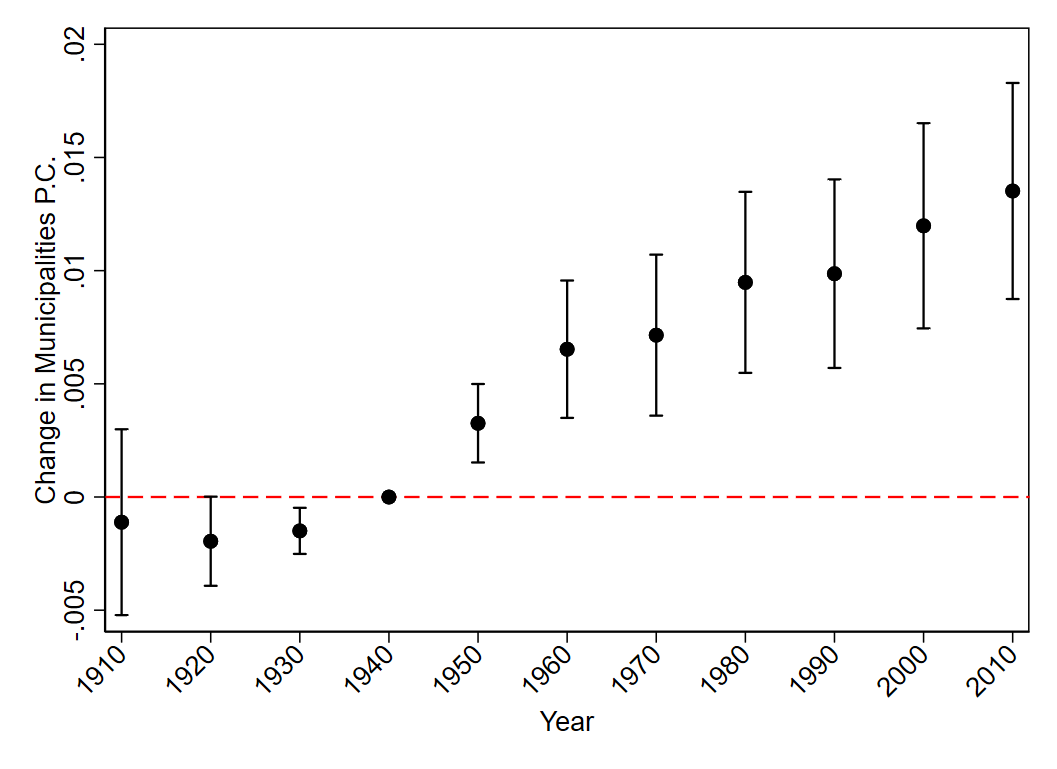
\includegraphics[width=\linewidth]{figures/F2a.png}
    \caption{Baseline Controls}
\end{subfigure}
\hfill
\begin{subfigure}[b]{0.65\textwidth}
    \centering
    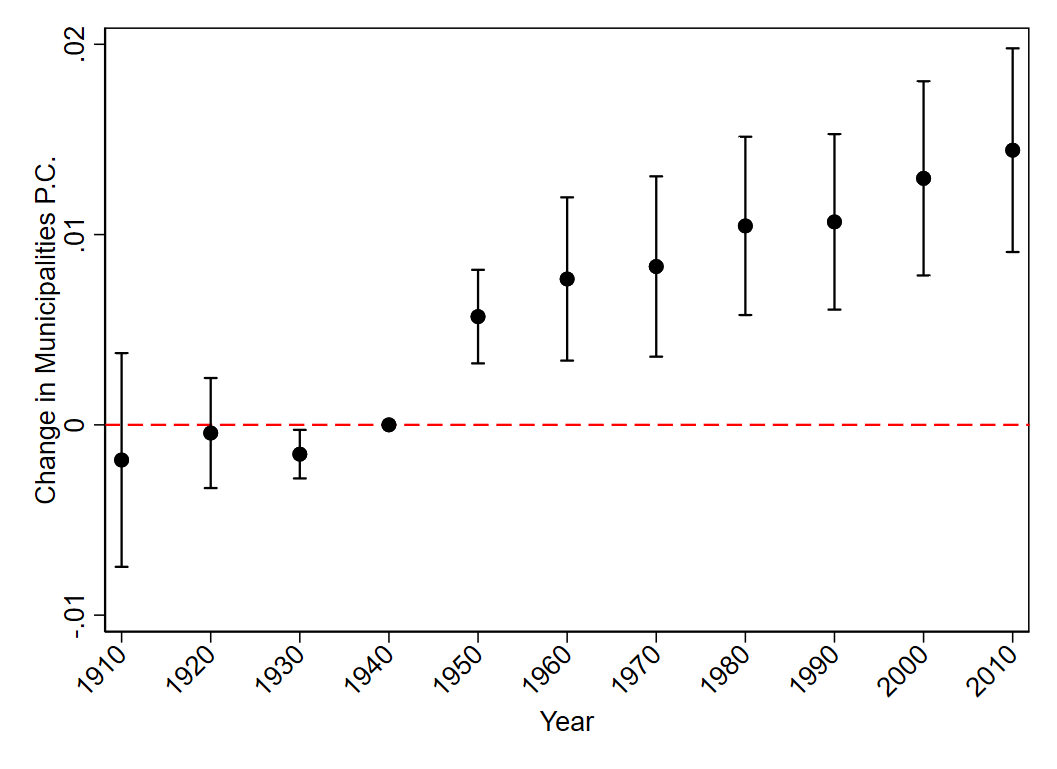
\includegraphics[width=\linewidth]{figures/F2b.png}
    \caption{Imbalanced Controls}
    \label{fig:sub2}
    \end{subfigure}
  
\end{figure}

\clearpage




%%%%%% TABLE 5

\begin{table}[htbp]
\centering
\scriptsize

\begin{threeparttable}
\caption{Dissolution of Incumbent Municipalities}
\label{tab:fragmech}
     \begin{tabularx}{\textwidth}{l*{4}{>{\centering\arraybackslash}X}} \toprule 
&\multicolumn{2}{c}{Disincorporations/Consolidations}&\multicolumn{2}{c}{Incumbent Municipality Land}\\\cmidrule(lr){2-3}\cmidrule(lr){4-5}
&\multicolumn{1}{c}{Raw}&\multicolumn{1}{c}{Zero Censored}&\multicolumn{1}{c}{$\Delta \log$ Land}&\multicolumn{1}{c}{$\Delta$ Prop. Incorporated}\\\cmidrule(lr){2-2}\cmidrule(lr){3-3}\cmidrule(lr){4-4}\cmidrule(lr){5-5}
&\multicolumn{1}{c}{(1)}&\multicolumn{1}{c}{(2)}&\multicolumn{1}{c}{(3)}&\multicolumn{1}{c}{(4)}\\
\cmidrule(lr){1-5}
\multicolumn{4}{l}{Panel A: First Stage}\\
\cmidrule(lr){1-5}
$\hat{GM}$      &    1.757***&    1.757***&    1.759***&    1.751***\\
                &  (0.316)   &  (0.316)   &  (0.315)   &  (0.315)   \\
\cmidrule(lr){1-5}
\multicolumn{4}{l}{Panel B: OLS 1940-1970}\\
\cmidrule(lr){1-5}
GM              &   -0.002   &   -0.002*  &   -0.026***&   -0.450*  \\
                &  (0.001)   &  (0.001)   &  (0.009)   &  (0.238)   \\
\cmidrule(lr){1-5}
\multicolumn{4}{l}{Panel C: 2SLS 1940-1970}\\
\cmidrule(lr){1-5}
GM              &   -0.005***&   -0.005***&   -0.066***&   -0.585***\\
                &  (0.001)   &  (0.001)   &  (0.006)   &  (0.166)   \\
\midrule
1940-70 Avg.    &     0.06   &     0.06   &     0.59   &     4.38   \\
\cmidrule(lr){1-5}
\multicolumn{4}{l}{Panel D: OLS 1940-2010}\\
\cmidrule(lr){1-5}
GM              &   -0.001   &   -0.001   &   -0.041***&   -0.785***\\
                &  (0.001)   &  (0.001)   &  (0.009)   &  (0.251)   \\
\cmidrule(lr){1-5}
\multicolumn{4}{l}{Panel E: 2SLS 1940-2010}\\
\cmidrule(lr){1-5}
GM              &   -0.003***&   -0.002** &   -0.073***&   -0.728***\\
                &  (0.001)   &  (0.001)   &  (0.006)   &  (0.206)   \\
\cmidrule(lr){1-5}
1940-2010 Avg.  &     0.08   &     0.08   &     0.95   &     8.48   \\
First Stage F-Stat&    30.93   &    30.93   &    31.10   &    30.85   \\
Observations    &      130   &      130   &      129   &      129   \\
 \bottomrule \end{tabularx}

    \end{threeparttable}
 \end{table}
\clearpage

\begin{table}[htbp]
\footnotesize
\centering \def\sym#1{\ifmmode^{#1}\else\(^{#1}\)\fi}  
\caption{Main results, Split on Occupation Scores of 1930-40 Black Migrants}\label{tab:occscore_split}
\begin{threeparttable}
\scriptsize 
    \begin{tabularx}{\textwidth}{l*{5}{>{\centering\arraybackslash}X}} \toprule \setlength{\tabcolsep}{15pt}
&\multicolumn{1}{c}{C. Goodman}&\multicolumn{3}{c}{Census of Governments}&\multicolumn{1}{c}{Census}\\\cmidrule(lr){2-2}\cmidrule(lr){3-5}\cmidrule(lr){6-6}
&\multicolumn{2}{c}{Municipalities}&\multicolumn{1}{c}{School districts}&\multicolumn{1}{c}{Special Districts}&\multicolumn{1}{c}{Main City Share}\\\cmidrule(lr){2-3}\cmidrule(lr){4-4}\cmidrule(lr){5-5}\cmidrule(lr){6-6}
&\multicolumn{1}{c}{(1)}&\multicolumn{1}{c}{(2)}&\multicolumn{1}{c}{(3)}&\multicolumn{1}{c}{(4)}&\multicolumn{1}{c}{(5)}\\
\cmidrule[1pt](lr){1-6}
\multicolumn{6}{c}{Black Migrant Differences \textit{Relative to other Black Migrants}}\\
\cmidrule[1pt](lr){1-6}
\multicolumn{5}{l}{Panel A: IV 1940-1970}\\
\cmidrule(lr){1-6}
GM  &    0.015*** &    0.020*** &    0.140* &    0.004 &    -1.708*** \\
                &  (0.003)  &  (0.004)  &  (0.080)  &  (0.005)  &  (0.114)  \\
GM X Above Median  &    -0.004 &    -0.013** &    0.390*** &    -0.009 &    0.169 \\
                &  (0.006)  &  (0.006)  &  (0.092)  &  (0.009)  &  (0.203)  \\
\cmidrule(lr){1-6}
\multicolumn{5}{l}{Panel B: IV 1940-2010}\\
\cmidrule(lr){1-6}
GM  &    0.021*** &    0.025*** &    0.150* &    0.026*** &    -1.854*** \\
                &  (0.004)  &  (0.005)  &  (0.083)  &  (0.005)  &  (0.189)  \\
GM X Above Median  &    0.001 &    -0.009 &    0.387*** &    -0.024** &    0.137 \\
                &  (0.006)  &  (0.006)  &  (0.093)  &  (0.010)  &  (0.220)  \\
\cmidrule(lr){1-6}
Below Median 1940-70 Avg. &      -0.357   &      -0.418   &      -8.768   &      0.536   &      -5.889   \\
Below Median 1940-2010 Avg. &      -0.475   &      -0.551   &      -9.114   &      0.720   &      -11.805   \\
Observations    &      97   &      978   &      978   &      978   &      978   \\
\cmidrule[1pt](lr){1-6}
\multicolumn{6}{c}{Black Migrant Differences \textit{Relative to Destination Residents}}\\
\cmidrule[1pt](lr){1-6}
\multicolumn{5}{l}{Panel C: IV 1940-1970}\\
\cmidrule(lr){1-6}
GM  &    0.008* &    0.013** &    -0.031 &    -0.005 &    -1.144*** \\
                &  (0.004)  &  (0.006)  &  (0.099)  &  (0.005)  &  (0.157)  \\
GM X Above Median  &    0.000 &    -0.006 &    1.799** &    0.027*** &    -1.159*** \\
                &  (0.004)  &  (0.005)  &  (0.887)  &  (0.010)  &  (0.246)  \\
\cmidrule(lr){1-6}
\multicolumn{5}{l}{Panel D: IV 1940-2010}\\
\cmidrule(lr){1-6}
GM  &    0.009 &    0.014* &    -0.038 &    0.002 &    -1.647*** \\
                &  (0.006)  &  (0.007)  &  (0.102)  &  (0.009)  &  (0.142)  \\
GM X Above Median  &    0.005 &    -0.003 &    1.839** &    0.037** &    -0.461** \\
                &  (0.005)  &  (0.006)  &  (0.909)  &  (0.015)  &  (0.224)  \\
\cmidrule(lr){1-6}
Below Median 1940-70 Avg. &      -0.316   &      -0.376   &      -7.345   &      0.505   &      -8.108   \\
Below Median 1940-2010 Avg. &      -0.427   &      -0.501   &      -7.623   &      0.705   &      -14.920   \\
Observations    &      957   &      918   &      918   &      918   &      918   \\
\bottomrule \end{tabularx}

 
    \end{threeparttable}
    \end{table}
\clearpage



%%%%%% FIGURE 2
\begin{figure}
    \captionsetup{justification=centering}
    \centering
    \caption{Most Incorporations in 1940-1970 are Mostly White, without large income differences}\label{fig:pcarrow_figure}
    \begin{subfigure}[b]{0.49\textwidth}
        	\centering
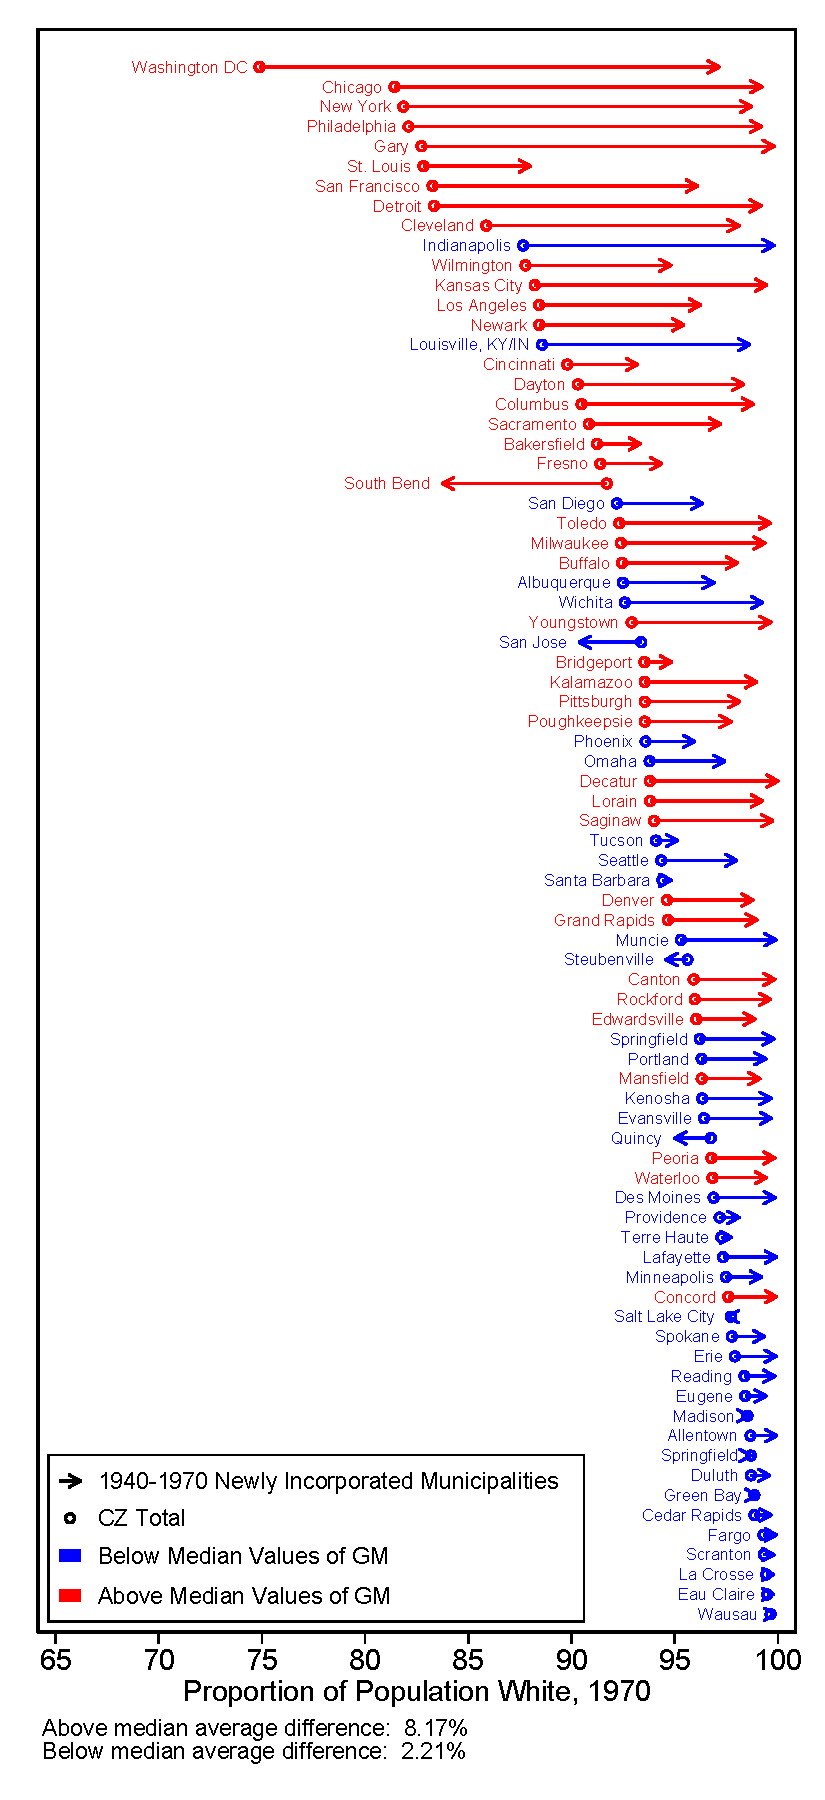
\includegraphics[width=.8\textwidth]{figures/F3a.pdf}
        \caption{Proportion of Population White, 1970}
    \end{subfigure}
    \begin{subfigure}[b]{0.49\textwidth}
            	\centering
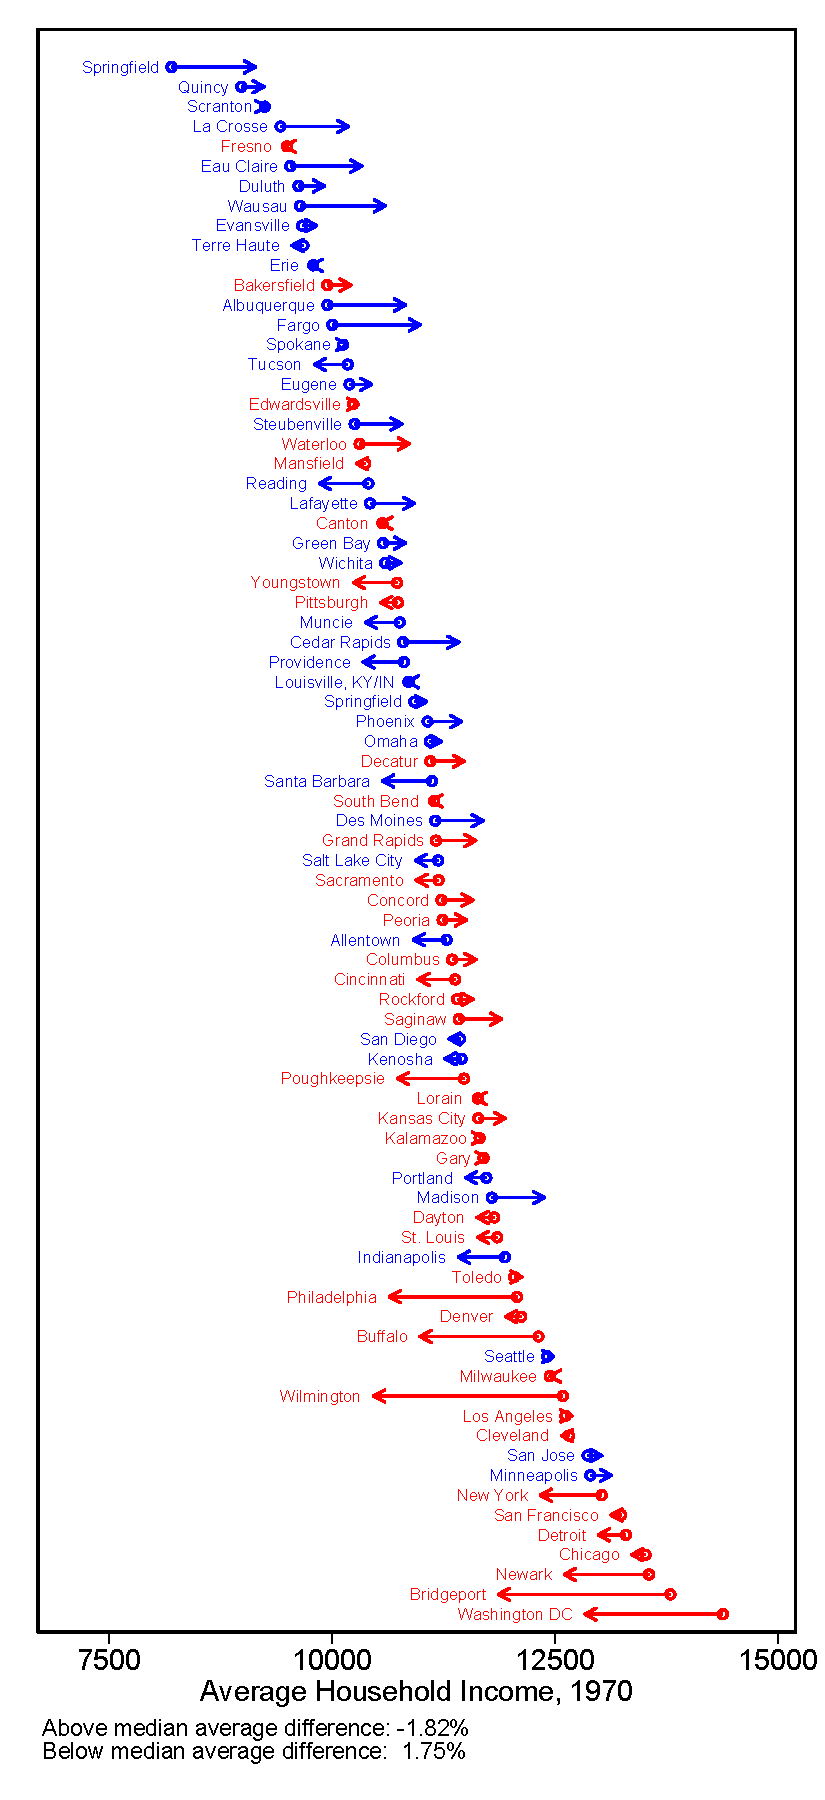
\includegraphics[width=.8\textwidth]{figures/F3b.pdf}
    \caption{Average Household Income, 1970}
    \end{subfigure}
 
\end{figure}

\begin{landscape}
\begin{table}[htbp]
\footnotesize
\centering \def\sym#1{\ifmmode^{#1}\else\(^{#1}\)\fi}  
\caption{Municipalities Incorporated between 1940 and 1970: Is racial exclusion a key motivator?}\label{tab:landuse}
\begin{threeparttable}
\scriptsize 
     \begin{tabularx}{\linewidth}{l*{8}{>{\centering\arraybackslash}X}} \toprule
                &\multicolumn{3}{c}{2010 Muni Characteristics}&\multicolumn{2}{c}{\shortstack{Percentage of \\ Municipal Revenues}}&\multicolumn{2}{c}{\shortstack{Percentage of \\ Municipal Land Uses}}&\multicolumn{1}{c}{\shortstack{Muni-District \\ Similarity}}\\\cmidrule(lr){2-4}\cmidrule(lr){5-6}\cmidrule(lr){7-8}\cmidrule(lr){9-9}
                &\multicolumn{1}{c}{(1)}&\multicolumn{1}{c}{(2)}&\multicolumn{1}{c}{(3)}&\multicolumn{1}{c}{(4)}&\multicolumn{1}{c}{(5)}&\multicolumn{1}{c}{(6)}&\multicolumn{1}{c}{(7)}&\multicolumn{1}{c}{(8)}\\
                &\multicolumn{1}{c}{\shortstack{Percentage \\ White}}&\multicolumn{1}{c}{\shortstack{Land Area}}&\multicolumn{1}{c}{\shortstack{2010 Household \\ Income}}&\multicolumn{1}{c}{\shortstack{Special \\ Assessments}}&\multicolumn{1}{c}{\shortstack{Fines and \\ Forfeitures}}&\multicolumn{1}{c}{\shortstack{Single \\ Family}}&\multicolumn{1}{c}{Apartments}&\multicolumn{1}{c}{\shortstack{Exclusive \\ District}}\\
\midrule
Above Median GM X Inc. 1940-70&    7.215*  & -121.168** &  -14.474***&   -1.539** &    0.583** &    9.612***&   -0.612***&    0.113*  \\
                &  (3.854)   & (57.019)   &  (4.949)   &  (0.684)   &  (0.275)   &  (3.084)   &  (0.182)   &  (0.067)   \\
\addlinespace
Above Median GM &  -15.989***&   35.029   &    7.937** &    0.190   &    0.539***&   -4.748*  &    0.720***&   -0.080   \\
                &  (3.016)   & (79.509)   &  (3.536)   &  (0.402)   &  (0.159)   &  (2.856)   &  (0.264)   &  (0.068)   \\
\addlinespace
Incorporated 1940-70&   -2.105   &  -79.763** &   22.302***&    1.267** &   -0.051   &   -1.586   &   -0.321***&   -0.128** \\
                &  (2.406)   & (35.494)   &  (3.845)   &  (0.609)   &  (0.194)   &  (2.587)   &  (0.088)   &  (0.064)   \\
\midrule
Omitted Category Avg.&    81.07   &   224.06   &    66.64   &     1.00   &     0.85   &    76.19   &     0.97   &     0.14   \\
Observations    &     7828   &     7841   &     7826   &     7732   &     7732   &     7714   &     7714   &     7577   \\
 \bottomrule \end{tabularx}


    \end{threeparttable}
    \end{table}
\end{landscape}

    
%%%%% TABLE 4
\begin{table}[htbp]
\centering \def\sym#1{\ifmmode^{#1}\else\(^{#1}\)\fi} 
\centering
\caption{Downstream: School Segregation and Achievement}\label{tab:seg}
\begin{threeparttable}
\footnotesize 
\begin{tabularx}{\textwidth}{l*{6}{>{\centering\arraybackslash}X}} \toprule
&\multicolumn{2}{c}{School District Segregation}&\multicolumn{4}{c}{School District Achievement}\\\cmidrule(lr){2-3}\cmidrule(lr){4-7}
                &\multicolumn{1}{c}{(1)}&\multicolumn{1}{c}{(2)}&\multicolumn{1}{c}{(3)}&\multicolumn{1}{c}{(4)}&\multicolumn{1}{c}{(5)}&\multicolumn{1}{c}{(6)}\\
                &\multicolumn{1}{c}{\shortstack{Variance \\ Ratio}}&\multicolumn{1}{c}{\shortstack{Dissimilarity \\ Index}}&\multicolumn{1}{c}{\shortstack{Interquartile \\ Range}}&\multicolumn{1}{c}{\shortstack{Variance}}&\multicolumn{1}{c}{\shortstack{Black \\ Exposure}}&\multicolumn{1}{c}{\shortstack{White \\ Exposure}}\\
\midrule
GM              &    0.006***&    0.001***&    0.005***&    0.001   &   -0.000   &    0.004** \\
                &  (0.002)   &  (0.000)   &  (0.001)   &  (0.001)   &  (0.002)   &  (0.002)   \\
\midrule
Dep. Var. Mean  &    0.253   &    0.283   &    0.318   &    0.072   &   -0.129   &    0.114   \\
Observations    &     1207   &     1207   &     1207   &     1207   &     1207   &     1207   \\
       \bottomrule \end{tabularx}

   
    \end{threeparttable}
    \end{table}
\clearpage
\section{Appendix}


\begin{table}[htbp]\centering 
 \begin{threeparttable} \caption{Balance Tests: 1940 Observables}\label{tab:balance}
   \begin{tabular}{l*{3}{c}} \toprule
&\multicolumn{2}{c}{$\widehat{GM}$}&\multicolumn{1}{c}{Mean}\\\cmidrule(lr){2-3}\cmidrule(lr){4-4}
&\multicolumn{1}{c}{(1)}&\multicolumn{1}{c}{(2)}&\multicolumn{1}{c}{(3)}\\
\midrule 
Average precipitation  &    0.426 & -0.046 & 14.460 \\
                &  (0.372)  &  (0.405)  &  (13.963)    \\
Average temperature  &    -0.632 & -0.798 & 38.974 \\
                &  (0.843)  &  (1.344)  &  (19.203)    \\
Number of Streams  &    3.102* & -16.327* & 59.899 \\
                &  (1.833)  &  (9.254)  &  (184.748)    \\
Coastal CZ  &    0.021* & 0.002 & 0.471 \\
                &  (0.011)  &  (0.017)  &  (0.501)    \\
Share of LF employed in manufacturing, 1940  &    0.228 & 1.166** & 25.022 \\
                &  (0.493)  &  (0.468)  &  (8.416)    \\
Meters of Railroad per Square Meter of Area, 1940  &    0.000 & 0.000 & 0.000 \\
                &  (0.000)  &  (0.000)  &  (0.000)    \\
Average Transport Cost out of CZ, 1920  &    -0.026 & -0.043 & 9.369 \\
                &  (0.038)  &  (0.040)  &  (3.003)    \\
Fraction of area incorporated  &    0.021* & 0.015 & 0.211 \\
                &  (0.012)  &  (0.010)  &  (0.223)    \\
Prop HS Grads, (25+)  &    0.000 & -0.004 & 0.263 \\
                &  (0.003)  &  (0.004)  &  (0.058)    \\
Prop College Grads, (25+)  &    0.002** & 0.001 & 0.054 \\
                &  (0.001)  &  (0.001)  &  (0.012)    \\
Average Income, 1940  &    16.323*** & 15.169* & 1163.222 \\
                &  (5.906)  &  (8.140)  &  (91.944)    \\
Population Density, 1940  &    25.980* & 22.455* & 256.867 \\
                &  (14.628)  &  (11.944)  &  (281.593)    \\
1930-40 Population Growth Rate  &    0.008*** & -0.001 & 0.076 \\
                &  (0.003)  &  (0.004)  &  (0.073)    \\
\bottomrule \end{tabular}
  \end{threeparttable} \end{table}

\begin{table}[htbp]\centering 
\begin{threeparttable} \caption{Pre-trends}
\label{tab:pretrends}
    \begin{tabularx}{\textwidth}{l*{5}{>{\centering\arraybackslash}X}} \toprule 
&\multicolumn{1}{c}{1900s}&\multicolumn{1}{c}{1910s}&\multicolumn{1}{c}{1920s}&\multicolumn{1}{c}{1930s}\\\cmidrule(lr){2-2}\cmidrule(lr){3-3}\cmidrule(lr){4-4}\cmidrule(lr){5-5}
&\multicolumn{1}{c}{(1)}&\multicolumn{1}{c}{(2)}&\multicolumn{1}{c}{(3)}&\multicolumn{1}{c}{(4)}\\
\midrule
\multicolumn{4}{l}{Panel A: $\Delta$ Municipalities Per Capita}\\
\cmidrule(lr){1-5}
$\widehat{GM}$  &   -0.005   &    0.013   &    0.003   &    0.004   \\
                &  (0.009)   &  (0.008)   &  (0.005)   &  (0.004)   \\
\midrule
Dep. var. mean  &     0.10   &    -0.02   &    -0.07   &    -0.05   \\
Dep. Var. Std Dev&     0.32   &     0.21   &     0.14   &     0.11   \\
Observations    &      130   &      130   &      130   &      130   \\
\midrule
\multicolumn{4}{l}{Panel B: \%$\Delta$ Population}\\
\cmidrule(lr){1-5}
$\widehat{GM}$  &   -6.052   &   -4.516***&   -3.938*  &   -0.427   \\
                &  (4.165)   &  (1.649)   &  (2.260)   &  (0.464)   \\
\midrule
Dep. var. mean  &    41.14   &    31.90   &    22.66   &     6.19   \\
Dep. Var. Std Dev&    41.43   &    27.21   &    19.59   &    10.67   \\
Observations    &      118   &      128   &      130   &      130   \\
\midrule
\multicolumn{5}{l}{Panel C: \%$\Delta$ Occupation Scores}\\
\cmidrule(lr){1-5}
$\widehat{GM}$  &   -0.006   &    0.042   &   -0.033   &    0.088   \\
                &  (0.106)   &  (0.044)   &  (0.068)   &  (0.068)   \\
\midrule
Dep. var. Avg.  &     1.75   &     3.14   &     0.00   &    -1.00   \\
Dep. var. Std Dev&     1.93   &     1.68   &     1.45   &     1.20   \\
Observations    &      118   &      127   &      129   &      130   \\
       \bottomrule \end{tabularx}
  \end{threeparttable}
\end{table}
\clearpage
\footnotesize
\begin{table}[htbp]
\footnotesize
\centering \def\sym#1{\ifmmode^{#1}\else\(^{#1}\)\fi}  \begin{threeparttable} \caption{Main effects, Township Outcome} \label{tab:main_effect_towns}
   \input{tables/TA3.tex}  \end{threeparttable}
 \end{table}
\clearpage

\begin{table}[htbp]
\centering \def\sym#1{\ifmmode^{#1}\else\(^{#1}\)\fi}  
\caption{Correlation Table}\label{tab:corr_matrix}
\begin{threeparttable}
      \begin{tabular}{l*{3}{c}} \toprule
& GM & $\Delta$ Municipalities P.C. \\
\cmidrule(lr){2-2} \cmidrule(lr){3-3}
&\multicolumn{1}{c}{(1)} & \multicolumn{1}{c}{(2)} \\
\cmidrule(lr){1-3}
 Pop. Growth 1940-70 & 0.167* & -0.322*** \\
\cmidrule(lr){1-3}
Observations & 130 & 130 \\
\bottomrule
\end{tabular}
 
    \end{threeparttable}
    \end{table}
\clearpage

\begin{table}[htbp]
\centering
\scriptsize

\begin{threeparttable}
\caption{Decomposition of Main Effect: Changes in Jurisdictions}
\label{tab:decomp_count}
       \begin{tabularx}{\textwidth}{l*{5}{>{\centering\arraybackslash}X}} \toprule \setlength{\tabcolsep}{15pt}
&\multicolumn{1}{c}{C. Goodman}&\multicolumn{3}{c}{Census of Governments}&\multicolumn{1}{c}{Census}\\\cmidrule(lr){2-2}\cmidrule(lr){3-5}\cmidrule(lr){6-6}
&\multicolumn{2}{c}{Municipalities}&\multicolumn{1}{c}{School districts}&\multicolumn{1}{c}{Special Districts}&\multicolumn{1}{c}{Main City Share}\\\cmidrule(lr){2-3}\cmidrule(lr){4-4}\cmidrule(lr){5-5}\cmidrule(lr){6-6}
&\multicolumn{1}{c}{(1)}&\multicolumn{1}{c}{(2)}&\multicolumn{1}{c}{(3)}&\multicolumn{1}{c}{(4)}&\multicolumn{1}{c}{(5)}\\
\cmidrule(lr){1-6}
\multicolumn{5}{l}{Panel A: First Stage}\\
\cmidrule(lr){1-6}
$\hat{GM}$      &    1.757***&    1.757***&    1.837***&    1.757***&    1.757***\\
                &  (0.316)   &  (0.316)   &  (0.332)   &  (0.316)   &  (0.316)   \\
\cmidrule(lr){1-6}
\multicolumn{5}{l}{Panel B: OLS 1940-1970}\\
\cmidrule(lr){1-6}
GM              &   -0.000   &    0.002   &    0.097   &   -0.001   &   -1.149***\\
                &  (0.002)   &  (0.003)   &  (0.076)   &  (0.015)   &  (0.396)   \\
\cmidrule(lr){1-6}
\multicolumn{5}{l}{Panel C: 2SLS 1940-1970}\\
\cmidrule(lr){1-6}
GM              &    0.002   &    0.006***&    0.162** &    0.052***&   -3.074***\\
                &  (0.002)   &  (0.002)   &  (0.068)   &  (0.014)   &  (0.347)   \\
\midrule
1940-70 Avg.    &     0.16   &     0.11   &   -12.38   &     1.40   &    17.22   \\
\cmidrule(lr){1-6}
\multicolumn{5}{l}{Panel D: OLS 1940-2010}\\
\cmidrule(lr){1-6}
GM              &   -0.001   &    0.000   &    0.094   &    0.002   &   -2.220***\\
                &  (0.003)   &  (0.004)   &  (0.077)   &  (0.023)   &  (0.785)   \\
\cmidrule(lr){1-6}
\multicolumn{5}{l}{Panel E: 2SLS 1940-2010}\\
\cmidrule(lr){1-6}
GM              &    0.001   &    0.004   &    0.154** &    0.113***&   -6.472***\\
                &  (0.003)   &  (0.003)   &  (0.069)   &  (0.029)   &  (0.983)   \\
\cmidrule(lr){1-6}
1940-2010 Avg.  &     0.23   &     0.15   &   -12.64   &     2.87   &    33.39   \\
1940 Avg.       &     1.48   &     1.61   &    14.05   &     0.88   &    32.78   \\
First Stage F-Stat&    30.93   &    30.93   &    30.61   &    30.93   &    30.93   \\
Observations    &      130   &      130   &      118   &      130   &      130   \\
 \bottomrule \end{tabularx}
 \end{threeparttable}
 \end{table}
\clearpage

\begin{table}[htbp]
\centering
\scriptsize

\begin{threeparttable}
\caption{Decomposition of Main Effect: Changes in Population}
\label{tab:decomp_pop}
         \begin{tabularx}{\textwidth}{l*{5}{>{\centering\arraybackslash}X}} \toprule \setlength{\tabcolsep}{15pt}
&\multicolumn{1}{c}{C. Goodman}&\multicolumn{3}{c}{Census of Governments}&\multicolumn{1}{c}{Census}\\\cmidrule(lr){2-2}\cmidrule(lr){3-5}\cmidrule(lr){6-6}
&\multicolumn{2}{c}{Municipalities}&\multicolumn{1}{c}{School districts}&\multicolumn{1}{c}{Special Districts}&\multicolumn{1}{c}{Main City Share}\\\cmidrule(lr){2-3}\cmidrule(lr){4-4}\cmidrule(lr){5-5}\cmidrule(lr){6-6}
&\multicolumn{1}{c}{(1)}&\multicolumn{1}{c}{(2)}&\multicolumn{1}{c}{(3)}&\multicolumn{1}{c}{(4)}&\multicolumn{1}{c}{(5)}\\
\cmidrule(lr){1-6}
\multicolumn{5}{l}{Panel A: First Stage}\\
\cmidrule(lr){1-6}
$\hat{GM}$      &    1.743***&    1.743***&    1.827***&    1.743***&    1.743***\\
                &  (0.317)   &  (0.317)   &  (0.331)   &  (0.317)   &  (0.317)   \\
\cmidrule(lr){1-6}
\multicolumn{5}{l}{Panel B: OLS 1940-1970}\\
\cmidrule(lr){1-6}
GM              &    0.003   &    0.003   &    0.004   &   -0.005   &    0.288   \\
                &  (0.003)   &  (0.004)   &  (0.004)   &  (0.009)   &  (0.332)   \\
\cmidrule(lr){1-6}
\multicolumn{5}{l}{Panel C: 2SLS 1940-1970}\\
\cmidrule(lr){1-6}
GM              &    0.006** &    0.005*  &    0.017***&   -0.042***&    1.553***\\
                &  (0.003)   &  (0.003)   &  (0.006)   &  (0.011)   &  (0.303)   \\
\midrule
1940-70 Avg.    &    -0.42   &    -0.43   &    -0.54   &    -0.76   &   -20.50   \\
\cmidrule(lr){1-6}
\multicolumn{5}{l}{Panel D: OLS 1940-2010}\\
\cmidrule(lr){1-6}
GM              &    0.006   &    0.006   &    0.007   &   -0.011   &    1.184   \\
                &  (0.005)   &  (0.005)   &  (0.005)   &  (0.021)   &  (0.749)   \\
\cmidrule(lr){1-6}
\multicolumn{5}{l}{Panel E: 2SLS 1940-2010}\\
\cmidrule(lr){1-6}
GM              &    0.009***&    0.007** &    0.025***&   -0.097***&    4.716***\\
                &  (0.003)   &  (0.003)   &  (0.007)   &  (0.028)   &  (0.947)   \\
\cmidrule(lr){1-6}
1940-2010 Avg.  &    -0.62   &    -0.64   &    -0.63   &    -1.82   &   -41.97   \\
1940 Avg.       &     1.48   &     1.61   &    14.05   &     0.88   &    32.78   \\
First Stage F-Stat&    30.23   &    30.23   &    30.44   &    30.23   &    30.23   \\
Observations    &      130   &      130   &      118   &      130   &      130   \\
 \bottomrule \end{tabularx}
\end{threeparttable}
 \end{table}
\clearpage

\begin{table}[htbp]
\footnotesize
\centering \def\sym#1{\ifmmode^{#1}\else\(^{#1}\)\fi}  \begin{threeparttable} \caption{Main effects, 1950-1970, avoiding the 1942 CoG measurement issues}
\label{tab:main_effect_1950_1970}
     \begin{tabularx}{\textwidth}{l*{5}{>{\centering\arraybackslash}X}} \toprule \setlength{\tabcolsep}{15pt}
&\multicolumn{1}{c}{C. Goodman}&\multicolumn{3}{c}{Census of Governments}&\multicolumn{1}{c}{Census}\\\cmidrule(lr){2-2}\cmidrule(lr){3-5}\cmidrule(lr){6-6}
&\multicolumn{2}{c}{Municipalities}&\multicolumn{1}{c}{School districts}&\multicolumn{1}{c}{Special Districts}&\multicolumn{1}{c}{Main City Share}\\\cmidrule(lr){2-3}\cmidrule(lr){4-4}\cmidrule(lr){5-5}\cmidrule(lr){6-6}
&\multicolumn{1}{c}{(1)}&\multicolumn{1}{c}{(2)}&\multicolumn{1}{c}{(3)}&\multicolumn{1}{c}{(4)}&\multicolumn{1}{c}{(5)}\\
\cmidrule(lr){1-6}
\multicolumn{5}{l}{Panel A: First Stage}\\
\cmidrule(lr){1-6}
$\hat{GM}$      &    1.743***&    1.743***&    1.827***&    1.743***&    1.743***\\
                &  (0.317)   &  (0.317)   &  (0.331)   &  (0.317)   &  (0.317)   \\
\cmidrule(lr){1-6}
\multicolumn{5}{l}{Panel B: OLS 1950-1970}\\
\cmidrule(lr){1-6}
GM              &    0.001   &    0.003   &    0.096** &    0.002   &   -0.730***\\
                &  (0.002)   &  (0.003)   &  (0.043)   &  (0.009)   &  (0.160)   \\
\cmidrule(lr){1-6}
\multicolumn{5}{l}{Panel C: 2SLS 1950-1970}\\
\cmidrule(lr){1-6}
GM              &    0.003   &    0.004** &    0.177***&    0.005   &   -1.383***\\
                &  (0.002)   &  (0.002)   &  (0.038)   &  (0.005)   &  (0.083)   \\
\midrule
1950-70 Avg.    &    -0.15   &    -0.18   &    -7.06   &     0.46   &    -2.45   \\
\cmidrule(lr){1-6}
\multicolumn{5}{l}{Panel D: OLS 1950-2010}\\
\cmidrule(lr){1-6}
GM              &    0.003   &    0.004   &    0.096** &   -0.000   &   -0.957***\\
                &  (0.003)   &  (0.004)   &  (0.043)   &  (0.008)   &  (0.205)   \\
\cmidrule(lr){1-6}
\multicolumn{5}{l}{Panel E: 2SLS 1950-2010}\\
\cmidrule(lr){1-6}
GM              &    0.004** &    0.005*  &    0.177***&    0.015** &   -1.685***\\
                &  (0.002)   &  (0.003)   &  (0.039)   &  (0.006)   &  (0.125)   \\
\cmidrule(lr){1-6}
1950-2010 Avg.  &    -0.28   &    -0.34   &    -7.41   &     0.86   &    -7.75   \\
1950 Avg.       &     1.38   &     1.46   &     8.19   &     1.07   &    31.95   \\
First Stage F-Stat&    30.23   &    30.23   &    30.44   &    30.23   &    30.23   \\
Observations    &      130   &      130   &      118   &      130   &      130   \\
 \bottomrule \end{tabularx}
 \end{threeparttable}  \end{table}
\clearpage

\begin{landscape}
\begin{table}[htbp]
\footnotesize
\centering \def\sym#1{\ifmmode^{#1}\else\(^{#1}\)\fi}  \begin{threeparttable} \caption{Effect on C. Goodman Municipalities, varying inclusion of imbalanced controls} \label{tab:cgoodman_balance_iter}
    \input{tables/TA8.tex} \end{threeparttable}
 \end{table}
\clearpage

\footnotesize
\begin{table}[htbp]
\footnotesize
\centering \def\sym#1{\ifmmode^{#1}\else\(^{#1}\)\fi}  \begin{threeparttable} \caption{Effect on CoG Municipalities, varying inclusion of imbalanced controls} \label{tab:gen_muni_balance_iter}
    \input{tables/TA9.tex} \end{threeparttable}
 \end{table}
\clearpage


\footnotesize
\begin{table}[htbp]
\footnotesize
\centering \def\sym#1{\ifmmode^{#1}\else\(^{#1}\)\fi}  \begin{threeparttable} \caption{Effect on School Districts, varying inclusion of imbalanced controls} \label{tab:schdist_ind_balance_iter}
     \begin{tabularx}{\linewidth}{l*{8}{>{\centering\arraybackslash}X}} \toprule
&\multicolumn{8}{c}{School Districts}\\\cmidrule(lr){2-9}
&\multicolumn{1}{c}{(1)}&\multicolumn{1}{c}{(2)}&\multicolumn{1}{c}{(3)}&\multicolumn{1}{c}{(4)}&\multicolumn{1}{c}{(5)}&\multicolumn{1}{c}{(6)}&\multicolumn{1}{c}{(7)}&\multicolumn{1}{c}{(8)}\\
\cmidrule(lr){1-9}
\multicolumn{8}{l}{Panel A: 2SLS 1940-70}\\
\cmidrule(lr){1-9}
GM              &    0.432***&    0.376***&    0.378***&    0.392***&    0.301***&    0.181** &    0.375***&    0.180** \\
                &  (0.046)   &  (0.062)   &  (0.053)   &  (0.047)   &  (0.070)   &  (0.073)   &  (0.053)   &  (0.072)   \\
\cmidrule(lr){1-9}
\multicolumn{8}{l}{Panel B: 2SLS 1940-2010}\\
\cmidrule(lr){1-9}
GM              &    0.445***&    0.382***&    0.388***&    0.404***&    0.304***&    0.182** &    0.385***&    0.180** \\
                &  (0.047)   &  (0.064)   &  (0.054)   &  (0.049)   &  (0.071)   &  (0.075)   &  (0.054)   &  (0.074)   \\
\cmidrule(lr){1-9}
Pop. Dens. Control&       No   &       No   &       No   &      Yes   &       No   &      Yes   &      Yes   &      Yes   \\
Avg. Income Control&       No   &       No   &      Yes   &       No   &      Yes   &       No   &      Yes   &      Yes   \\
Share Mfg. Control&       No   &      Yes   &       No   &       No   &      Yes   &      Yes   &       No   &      Yes   \\
 \bottomrule \end{tabularx}
 \end{threeparttable}
 \end{table}
\clearpage


\footnotesize
\begin{table}[htbp]
\footnotesize
\centering \def\sym#1{\ifmmode^{#1}\else\(^{#1}\)\fi}  \begin{threeparttable} \caption{Effect on Special Districts, varying inclusion of imbalanced controls} \label{tab:spdist_balance_iter}
    \input{tables/TA11.tex} \end{threeparttable}
 \end{table}
\clearpage


\footnotesize
\begin{table}[htbp]
\footnotesize
\centering \def\sym#1{\ifmmode^{#1}\else\(^{#1}\)\fi}  \begin{threeparttable} \caption{Effect on Main City Share, varying inclusion of imbalanced controls} \label{tab:totfrac_balance_iter}
     \begin{tabularx}{\linewidth}{l*{8}{>{\centering\arraybackslash}X}} \toprule
&\multicolumn{8}{c}{Main City Share}\\\cmidrule(lr){2-9}
&\multicolumn{1}{c}{(1)}&\multicolumn{1}{c}{(2)}&\multicolumn{1}{c}{(3)}&\multicolumn{1}{c}{(4)}&\multicolumn{1}{c}{(5)}&\multicolumn{1}{c}{(6)}&\multicolumn{1}{c}{(7)}&\multicolumn{1}{c}{(8)}\\
\cmidrule(lr){1-9}
\multicolumn{8}{l}{Panel A: 2SLS 1940-70}\\
\cmidrule(lr){1-9}
GM              &   -1.429***&   -1.540***&   -1.449***&   -1.374***&   -1.615***&   -1.482***&   -1.456***&   -1.573***\\
                &  (0.052)   &  (0.067)   &  (0.065)   &  (0.053)   &  (0.092)   &  (0.079)   &  (0.064)   &  (0.090)   \\
\cmidrule(lr){1-9}
\multicolumn{8}{l}{Panel B: 2SLS 1940-2010}\\
\cmidrule(lr){1-9}
GM              &   -1.671***&   -1.700***&   -1.803***&   -1.665***&   -1.893***&   -1.702***&   -1.808***&   -1.858***\\
                &  (0.085)   &  (0.107)   &  (0.099)   &  (0.090)   &  (0.140)   &  (0.130)   &  (0.094)   &  (0.134)   \\
\cmidrule(lr){1-9}
Pop. Dens. Control&       No   &       No   &       No   &      Yes   &       No   &      Yes   &      Yes   &      Yes   \\
Avg. Income Control&       No   &       No   &      Yes   &       No   &      Yes   &       No   &      Yes   &      Yes   \\
Share Mfg. Control&       No   &      Yes   &       No   &       No   &      Yes   &      Yes   &       No   &      Yes   \\
 \bottomrule \end{tabularx}
 \end{threeparttable}
 \end{table}
\clearpage

\end{landscape}

\footnotesize
\begin{table}[htbp]
\footnotesize
\centering \def\sym#1{\ifmmode^{#1}\else\(^{#1}\)\fi}  \begin{threeparttable} \caption{Main effects, 1940-1970, without controls for imbalanced baseline covariates}  \label{tab:main_effect_noctrl}
     \begin{tabularx}{\textwidth}{l*{5}{>{\centering\arraybackslash}X}} \toprule \setlength{\tabcolsep}{15pt}
&\multicolumn{1}{c}{C. Goodman}&\multicolumn{3}{c}{Census of Governments}&\multicolumn{1}{c}{Census}\\\cmidrule(lr){2-2}\cmidrule(lr){3-5}\cmidrule(lr){6-6}
&\multicolumn{2}{c}{Municipalities}&\multicolumn{1}{c}{School districts}&\multicolumn{1}{c}{Special Districts}&\multicolumn{1}{c}{Main City Share}\\\cmidrule(lr){2-3}\cmidrule(lr){4-4}\cmidrule(lr){5-5}\cmidrule(lr){6-6}
&\multicolumn{1}{c}{(1)}&\multicolumn{1}{c}{(2)}&\multicolumn{1}{c}{(3)}&\multicolumn{1}{c}{(4)}&\multicolumn{1}{c}{(5)}\\
\cmidrule(lr){1-6}
\multicolumn{5}{l}{Panel A: First Stage}\\
\cmidrule(lr){1-6}
$\hat{GM}$      &    2.545***&    2.545***&    2.680***&    2.545***&    2.545***\\
                &  (0.366)   &  (0.366)   &  (0.412)   &  (0.366)   &  (0.366)   \\
\cmidrule(lr){1-6}
\multicolumn{5}{l}{Panel B: OLS 1940-1970}\\
\cmidrule(lr){1-6}
GM              &    0.004   &    0.007** &    0.350***&   -0.026***&   -1.024***\\
                &  (0.003)   &  (0.003)   &  (0.087)   &  (0.008)   &  (0.142)   \\
\cmidrule(lr){1-6}
\multicolumn{5}{l}{Panel C: 2SLS 1940-1970}\\
\cmidrule(lr){1-6}
GM              &    0.007***&    0.011***&    0.432***&   -0.017***&   -1.424***\\
                &  (0.002)   &  (0.002)   &  (0.046)   &  (0.003)   &  (0.052)   \\
\midrule
1940-70 Avg.    &    -0.26   &    -0.33   &   -12.91   &     0.64   &    -3.28   \\
\cmidrule(lr){1-6}
\multicolumn{5}{l}{Panel D: OLS 1940-2010}\\
\cmidrule(lr){1-6}
GM              &    0.011***&    0.014***&    0.362***&   -0.038***&   -1.239***\\
                &  (0.004)   &  (0.004)   &  (0.088)   &  (0.008)   &  (0.188)   \\
\cmidrule(lr){1-6}
\multicolumn{5}{l}{Panel E: 2SLS 1940-2010}\\
\cmidrule(lr){1-6}
GM              &    0.013***&    0.017***&    0.445***&   -0.022***&   -1.671***\\
                &  (0.002)   &  (0.003)   &  (0.047)   &  (0.005)   &  (0.085)   \\
\cmidrule(lr){1-6}
1940-2010 Avg.  &    -0.39   &    -0.49   &   -13.27   &     1.05   &    -8.58   \\
1940 Avg.       &     1.48   &     1.61   &    14.05   &     0.88   &    32.78   \\
First Stage F-Stat&    48.25   &    48.25   &    42.37   &    48.25   &    48.25   \\
Observations    &      130   &      130   &      118   &      130   &      130   \\
 \bottomrule \end{tabularx}
 \end{threeparttable}
 \end{table}
\clearpage


\footnotesize
\begin{table}[htbp]
\centering
\scriptsize
\begin{threeparttable}
\caption{Main Effects, including all baseline covariates}
\label{tab:allctrls}
        \begin{tabularx}{\textwidth}{l*{5}{>{\centering\arraybackslash}X}} \toprule \setlength{\tabcolsep}{15pt}
&\multicolumn{1}{c}{C. Goodman}&\multicolumn{3}{c}{Census of Governments}&\multicolumn{1}{c}{Census}\\\cmidrule(lr){2-2}\cmidrule(lr){3-5}\cmidrule(lr){6-6}
&\multicolumn{2}{c}{Municipalities}&\multicolumn{1}{c}{School districts}&\multicolumn{1}{c}{Special Districts}&\multicolumn{1}{c}{Main City Share}\\\cmidrule(lr){2-3}\cmidrule(lr){4-4}\cmidrule(lr){5-5}\cmidrule(lr){6-6}
&\multicolumn{1}{c}{(1)}&\multicolumn{1}{c}{(2)}&\multicolumn{1}{c}{(3)}&\multicolumn{1}{c}{(4)}&\multicolumn{1}{c}{(5)}\\
\cmidrule(lr){1-6}
\multicolumn{5}{l}{Panel A: First Stage}\\
\cmidrule(lr){1-6}
$\hat{GM}$      &    1.599***&    1.599***&    1.836***&    1.599***&    1.599***\\
                &  (0.243)   &  (0.243)   &  (0.254)   &  (0.243)   &  (0.243)   \\
\cmidrule(lr){1-6}
\multicolumn{5}{l}{Panel B: OLS 1940-1970}\\
\cmidrule(lr){1-6}
GM              &    0.005*  &    0.006*  &    0.057   &   -0.011   &   -1.110***\\
                &  (0.003)   &  (0.004)   &  (0.097)   &  (0.010)   &  (0.161)   \\
\cmidrule(lr){1-6}
\multicolumn{5}{l}{Panel C: 2SLS 1940-1970}\\
\cmidrule(lr){1-6}
GM              &    0.013***&    0.014***&    0.176** &    0.010   &   -1.831***\\
                &  (0.003)   &  (0.003)   &  (0.081)   &  (0.008)   &  (0.130)   \\
\midrule
1940-70 Avg.    &    -0.26   &    -0.33   &   -12.91   &     0.64   &    -3.30   \\
\cmidrule(lr){1-6}
\multicolumn{5}{l}{Panel D: OLS 1940-2010}\\
\cmidrule(lr){1-6}
GM              &    0.007   &    0.007   &    0.057   &   -0.016   &   -1.361***\\
                &  (0.005)   &  (0.005)   &  (0.099)   &  (0.013)   &  (0.214)   \\
\cmidrule(lr){1-6}
\multicolumn{5}{l}{Panel E: 2SLS 1940-2010}\\
\cmidrule(lr){1-6}
GM              &    0.018***&    0.017***&    0.174** &    0.038***&   -2.096***\\
                &  (0.004)   &  (0.004)   &  (0.083)   &  (0.010)   &  (0.179)   \\
\cmidrule(lr){1-6}
1940-2010 Avg.  &    -0.39   &    -0.49   &   -13.27   &     1.05   &    -8.58   \\
1940 Avg.       &     1.48   &     1.61   &    14.05   &     0.88   &    32.78   \\
First Stage F-Stat&    43.29   &    43.29   &    52.17   &    43.29   &    43.29   \\
Observations    &      130   &      130   &      118   &      130   &      130   \\
 \bottomrule \end{tabularx}
 \end{threeparttable}
 \end{table}
\clearpage


\begin{table}[htbp]
\centering
\tiny
\begin{threeparttable}
\caption{Main Effects, varying inclusion of all baseline controls}
\label{tab:varyctrl}
     \begin{tabularx}{\textwidth}{l*{5}{>{\centering\arraybackslash}X}} \toprule \setlength{\tabcolsep}{15pt}
&\multicolumn{1}{c}{C. Goodman}&\multicolumn{3}{c}{Census of Governments}&\multicolumn{1}{c}{Census}\\\cmidrule(lr){2-2}\cmidrule(lr){3-5}\cmidrule(lr){6-6}
&\multicolumn{2}{c}{Municipalities}&\multicolumn{1}{c}{School districts}&\multicolumn{1}{c}{Special Districts}&\multicolumn{1}{c}{Main City Share}\\\cmidrule(lr){2-3}\cmidrule(lr){4-4}\cmidrule(lr){5-5}\cmidrule(lr){6-6}
&\multicolumn{1}{c}{(1)}&\multicolumn{1}{c}{(2)}&\multicolumn{1}{c}{(3)}&\multicolumn{1}{c}{(4)}&\multicolumn{1}{c}{(5)}\\
\cmidrule(lr){1-6}
\multicolumn{5}{l}{Balance Control Included}\\
\cmidrule(lr){1-6}
None  &    0.007*** &    0.011*** &    0.432*** &    -0.017*** &    -1.429*** \\
                &  (0.000)  &  (0.000)  &  (0.002)  &  (0.000)  &  (0.003)  \\
\cmidrule(lr){1-6}
Average precipitation  &    0.007*** &    0.011*** &    0.430*** &    -0.017*** &    -1.428*** \\
                &  (0.002)  &  (0.002)  &  (0.047)  &  (0.003)  &  (0.051)  \\
Average temperature  &    0.007*** &    0.010*** &    0.438*** &    -0.015*** &    -1.428*** \\
                &  (0.002)  &  (0.002)  &  (0.046)  &  (0.003)  &  (0.052)  \\
Number of Streams  &    0.008*** &    0.012*** &    0.408*** &    -0.020*** &    -1.392*** \\
                &  (0.002)  &  (0.002)  &  (0.044)  &  (0.003)  &  (0.055)  \\
Coastal CZ  &    0.007*** &    0.011*** &    0.431*** &    -0.017*** &    -1.429*** \\
                &  (0.002)  &  (0.002)  &  (0.047)  &  (0.003)  &  (0.051)  \\
Share of LF employed in manufacturing, 1940  &    0.008*** &    0.011*** &    0.375*** &    -0.014*** &    -1.540*** \\
                &  (0.002)  &  (0.003)  &  (0.062)  &  (0.004)  &  (0.067)  \\
Meters of Railroad per Square Meter of Area, 1940  &    0.007*** &    0.011*** &    0.410*** &    -0.022*** &    -1.490*** \\
                &  (0.002)  &  (0.002)  &  (0.048)  &  (0.004)  &  (0.053)  \\
Average Transport Cost out of CZ, 1920  &    0.007*** &    0.011*** &    0.430*** &    -0.018*** &    -1.442*** \\
                &  (0.002)  &  (0.002)  &  (0.046)  &  (0.003)  &  (0.052)  \\
Fraction of area incorporated  &    0.006*** &    0.009*** &    0.398*** &    -0.012*** &    -1.377*** \\
                &  (0.002)  &  (0.002)  &  (0.046)  &  (0.003)  &  (0.052)  \\
Prop HS Grads, (25+)  &    0.006*** &    0.010*** &    0.459*** &    -0.018*** &    -1.487*** \\
                &  (0.002)  &  (0.002)  &  (0.048)  &  (0.004)  &  (0.058)  \\
Prop College Grads, (25+)  &    0.007*** &    0.011*** &    0.429*** &    -0.015*** &    -1.402*** \\
                &  (0.002)  &  (0.002)  &  (0.047)  &  (0.004)  &  (0.056)  \\
Average Income, 1940  &    0.008*** &    0.011*** &    0.381*** &    -0.004 &    -1.449*** \\
                &  (0.002)  &  (0.003)  &  (0.052)  &  (0.005)  &  (0.065)  \\
Population Density, 1940  &    0.005*** &    0.009*** &    0.392*** &    -0.011*** &    -1.374*** \\
                &  (0.002)  &  (0.002)  &  (0.047)  &  (0.003)  &  (0.053)  \\
1930-40 Population Growth Rate  &    0.007*** &    0.011*** &    0.432*** &    -0.018*** &    -1.438*** \\
                &  (0.002)  &  (0.002)  &  (0.047)  &  (0.004)  &  (0.053)  \\
\cmidrule(lr){1-6}
Imbalanced  &    0.008*** &    0.011*** &    0.179** &    0.009 &    -1.573*** \\
                &  (0.003)  &  (0.003)  &  (0.072)  &  (0.006)  &  (0.090)  \\
All  &    0.013*** &    0.014*** &    0.176** &    0.010 &    -1.831*** \\
                &  (0.003)  &  (0.003)  &  (0.081)  &  (0.008)  &  (0.130)  \\
\cmidrule(lr){1-6}
Observations    &      130   &      130   &      118   &      130   &      130   \\
\bottomrule \end{tabularx}
\end{threeparttable}
 \end{table}
\clearpage



\begin{table}[htbp]\centering 
 \begin{threeparttable} \caption{Balance Tests: 1940 Observables using the percentile instrument and endogenous regressor}\label{tab:balance_pctile}
    \begin{tabular}{l*{3}{c}} \toprule
&\multicolumn{2}{c}{Percentile  $\widehat{GM}$}&\multicolumn{1}{c}{Mean}\\\cmidrule(lr){2-3}\cmidrule(lr){4-4}
&\multicolumn{1}{c}{(1)}&\multicolumn{1}{c}{(2)}&\multicolumn{1}{c}{(3)}\\
\midrule 
Average precipitation  &    0.110* & 0.113* & 14.460 \\
                &  (0.062)  &  (0.064)  &  (13.963)    \\
Average temperature  &    -0.088 & -0.092 & 38.974 \\
                &  (0.097)  &  (0.097)  &  (19.203)    \\
Number of Streams  &    1.632** & 1.325* & 59.899 \\
                &  (0.805)  &  (0.743)  &  (184.748)    \\
Coastal CZ  &    0.003 & 0.002 & 0.471 \\
                &  (0.002)  &  (0.002)  &  (0.501)    \\
Share of LF employed in manufacturing, 1940  &    0.032 & 0.078 & 25.022 \\
                &  (0.050)  &  (0.051)  &  (8.416)    \\
Meters of Railroad per Square Meter of Area, 1940  &    0.000 & 0.000* & 0.000 \\
                &  (0.000)  &  (0.000)  &  (0.000)    \\
Average Transport Cost out of CZ, 1920  &    -0.011* & -0.016** & 9.369 \\
                &  (0.006)  &  (0.007)  &  (3.003)    \\
Fraction of area incorporated  &    0.003** & 0.003* & 0.211 \\
                &  (0.002)  &  (0.002)  &  (0.223)    \\
Prop HS Grads, (25+)  &    -0.000 & -0.001 & 0.263 \\
                &  (0.000)  &  (0.000)  &  (0.058)    \\
Prop College Grads, (25+)  &    0.000* & -0.000 & 0.054 \\
                &  (0.000)  &  (0.000)  &  (0.012)    \\
Average Income, 1940  &    1.839*** & 1.421** & 1163.222 \\
                &  (0.614)  &  (0.689)  &  (91.944)    \\
Population Density, 1940  &    4.600** & 4.816** & 256.867 \\
                &  (1.948)  &  (1.894)  &  (281.593)    \\
1930-40 Population Growth Rate  &    0.001*** & 0.000 & 0.076 \\
                &  (0.000)  &  (0.000)  &  (0.073)    \\
\bottomrule \end{tabular}
 \end{threeparttable} \end{table}


\begin{table}[htbp]
\footnotesize
\centering \def\sym#1{\ifmmode^{#1}\else\(^{#1}\)\fi}  \begin{threeparttable} \caption{Main effects, 1940-1970, using percentile transformation of instrument and endogenous regressor}\label{tab:main_effect_pctile}
     \begin{tabularx}{\textwidth}{l*{5}{>{\centering\arraybackslash}X}} \toprule \setlength{\tabcolsep}{15pt}
&\multicolumn{1}{c}{C. Goodman}&\multicolumn{3}{c}{Census of Governments}&\multicolumn{1}{c}{Census}\\\cmidrule(lr){2-2}\cmidrule(lr){3-5}\cmidrule(lr){6-6}
&\multicolumn{2}{c}{Municipalities}&\multicolumn{1}{c}{School districts}&\multicolumn{1}{c}{Special Districts}&\multicolumn{1}{c}{Main City Share}\\\cmidrule(lr){2-3}\cmidrule(lr){4-4}\cmidrule(lr){5-5}\cmidrule(lr){6-6}
&\multicolumn{1}{c}{(1)}&\multicolumn{1}{c}{(2)}&\multicolumn{1}{c}{(3)}&\multicolumn{1}{c}{(4)}&\multicolumn{1}{c}{(5)}\\
\cmidrule(lr){1-6}
\multicolumn{5}{l}{Panel A: First Stage}\\
\cmidrule(lr){1-6}
Percentile $\widehat{GM}$&    0.481***&    0.481***&    0.340***&    0.481***&    0.481***\\
                &  (0.119)   &  (0.119)   &  (0.118)   &  (0.119)   &  (0.119)   \\
\cmidrule(lr){1-6}
\multicolumn{5}{l}{Panel B: OLS 1940-1970}\\
\cmidrule(lr){1-6}
Percentile GM   &   -0.001   &    0.000   &    0.099***&   -0.009***&   -0.185***\\
                &  (0.001)   &  (0.001)   &  (0.034)   &  (0.003)   &  (0.057)   \\
\cmidrule(lr){1-6}
\multicolumn{5}{l}{Panel C: 2SLS 1940-1970}\\
\cmidrule(lr){1-6}
Percentile GM   &    0.001   &    0.002   &    0.342***&   -0.002   &   -0.427***\\
                &  (0.002)   &  (0.002)   &  (0.127)   &  (0.007)   &  (0.122)   \\
\midrule
1940-70 Avg.    &    -0.26   &    -0.33   &   -12.91   &     0.64   &    -3.28   \\
\cmidrule(lr){1-6}
\multicolumn{5}{l}{Panel D: OLS 1940-2010}\\
\cmidrule(lr){1-6}
Percentile GM   &    0.001   &    0.003   &    0.101***&   -0.018***&   -0.283***\\
                &  (0.002)   &  (0.002)   &  (0.035)   &  (0.004)   &  (0.086)   \\
\cmidrule(lr){1-6}
\multicolumn{5}{l}{Panel E: 2SLS 1940-2010}\\
\cmidrule(lr){1-6}
Percentile GM   &    0.006*  &    0.007** &    0.351***&   -0.006   &   -0.625***\\
                &  (0.003)   &  (0.003)   &  (0.129)   &  (0.008)   &  (0.162)   \\
\cmidrule(lr){1-6}
1940-2010 Avg.  &    -0.39   &    -0.49   &   -13.27   &     1.05   &    -8.58   \\
1940 Avg.       &     1.48   &     1.61   &    14.05   &     0.88   &    32.78   \\
First State F-Stat&    16.35   &    16.35   &     8.27   &    16.35   &    16.35   \\
Observations    &      130   &      130   &      118   &      130   &      130   \\
 \bottomrule \end{tabularx}

 \end{threeparttable} 
\end{table}
\clearpage



\footnotesize
\begin{table}[htbp]
\footnotesize
\centering \def\sym#1{\ifmmode^{#1}\else\(^{#1}\)\fi}  \begin{threeparttable} \caption{Main effects, including European migration control} \label{tab:main_effect_eurmig}
     \begin{tabularx}{\textwidth}{l*{5}{>{\centering\arraybackslash}X}} \toprule \setlength{\tabcolsep}{15pt}
&\multicolumn{1}{c}{C. Goodman}&\multicolumn{3}{c}{Census of Governments}&\multicolumn{1}{c}{Census}\\\cmidrule(lr){2-2}\cmidrule(lr){3-5}\cmidrule(lr){6-6}
&\multicolumn{2}{c}{Municipalities}&\multicolumn{1}{c}{School districts}&\multicolumn{1}{c}{Special Districts}&\multicolumn{1}{c}{Main City Share}\\\cmidrule(lr){2-3}\cmidrule(lr){4-4}\cmidrule(lr){5-5}\cmidrule(lr){6-6}
&\multicolumn{1}{c}{(1)}&\multicolumn{1}{c}{(2)}&\multicolumn{1}{c}{(3)}&\multicolumn{1}{c}{(4)}&\multicolumn{1}{c}{(5)}\\
\cmidrule(lr){1-6}
\multicolumn{5}{l}{Panel A: First Stage}\\
\cmidrule(lr){1-6}
$\hat{GM}$      &    1.868***&    1.868***&    2.075***&    1.868***&    1.868***\\
                &  (0.331)   &  (0.331)   &  (0.352)   &  (0.331)   &  (0.331)   \\
\cmidrule(lr){1-6}
\multicolumn{5}{l}{Panel B: OLS 1940-1970}\\
\cmidrule(lr){1-6}
GM              &    0.003   &    0.005   &    0.106   &   -0.005   &   -0.901***\\
                &  (0.003)   &  (0.004)   &  (0.078)   &  (0.010)   &  (0.172)   \\
\cmidrule(lr){1-6}
\multicolumn{5}{l}{Panel C: 2SLS 1940-1970}\\
\cmidrule(lr){1-6}
GM              &    0.010***&    0.014***&    0.130** &    0.000   &   -1.554***\\
                &  (0.003)   &  (0.003)   &  (0.065)   &  (0.006)   &  (0.088)   \\
\midrule
1940-70 Avg.    &    -0.26   &    -0.33   &   -12.91   &     0.64   &    -3.28   \\
\cmidrule(lr){1-6}
\multicolumn{5}{l}{Panel D: OLS 1940-2010}\\
\cmidrule(lr){1-6}
GM              &    0.005   &    0.006   &    0.106   &   -0.007   &   -1.140***\\
                &  (0.005)   &  (0.005)   &  (0.079)   &  (0.008)   &  (0.216)   \\
\cmidrule(lr){1-6}
\multicolumn{5}{l}{Panel E: 2SLS 1940-2010}\\
\cmidrule(lr){1-6}
GM              &    0.013***&    0.015***&    0.132** &    0.013** &   -1.767***\\
                &  (0.003)   &  (0.004)   &  (0.067)   &  (0.006)   &  (0.121)   \\
\cmidrule(lr){1-6}
1940-2010 Avg.  &    -0.39   &    -0.49   &   -13.27   &     1.05   &    -8.58   \\
1940 Avg.       &     1.48   &     1.61   &    14.05   &     0.88   &    32.78   \\
First Stage F-Stat&    31.91   &    31.91   &    34.76   &    31.91   &    31.91   \\
Observations    &      130   &      130   &      118   &      130   &      130   \\
 \bottomrule \end{tabularx}
 \end{threeparttable}
 \end{table}
\clearpage


\begin{table}[htbp]\centering 
 \begin{threeparttable} \caption{White Instrument Balance Tests: 1940 Observables}\label{tab:balance_white}
    \begin{tabular}{l*{3}{c}} \toprule
&\multicolumn{2}{c}{$\widehat{WM}$}&\multicolumn{1}{c}{Mean}\\\cmidrule(lr){2-3}\cmidrule(lr){4-4}
&\multicolumn{1}{c}{(1)}&\multicolumn{1}{c}{(2)}&\multicolumn{1}{c}{(3)}\\
\midrule 
Average precipitation  &    0.280 & 0.346 & 14.460 \\
                &  (0.604)  &  (0.712)  &  (13.963)    \\
Average temperature  &    -0.274 & 0.775 & 38.974 \\
                &  (1.414)  &  (1.576)  &  (19.203)    \\
Number of Streams  &    29.128 & 36.670 & 496.718 \\
                &  (21.879)  &  (27.573)  &  (346.648)    \\
Coastal CZ  &    -0.017 & -0.037** & 0.471 \\
                &  (0.013)  &  (0.018)  &  (0.501)    \\
Share of LF employed in manufacturing, 1940  &    0.740 & 2.022*** & 25.022 \\
                &  (0.534)  &  (0.598)  &  (8.416)    \\
Meters of Railroad per Square Meter of Area, 1940  &    -0.000 & 0.000 & 0.000 \\
                &  (0.000)  &  (0.000)  &  (0.000)    \\
Average Transport Cost out of CZ, 1920  &    -0.005 & 0.012 & 9.369 \\
                &  (0.049)  &  (0.058)  &  (3.003)    \\
Fraction of area incorporated  &    -0.021* & -0.025* & 0.209 \\
                &  (0.011)  &  (0.014)  &  (0.227)    \\
Prop HS Grads, (25+)  &    -0.007*** & -0.015*** & 0.263 \\
                &  (0.002)  &  (0.003)  &  (0.058)    \\
Prop College Grads, (25+)  &    -0.002*** & -0.005*** & 0.054 \\
                &  (0.001)  &  (0.001)  &  (0.012)    \\
Average Income, 1940  &    -12.063** & -17.409* & 1163.358 \\
                &  (6.038)  &  (9.749)  &  (91.626)    \\
Population Density, 1940  &    -21.373* & -22.418 & 253.317 \\
                &  (12.213)  &  (16.272)  &  (281.826)    \\
1930-40 Population Growth Rate  &    0.008* & -0.011** & 0.076 \\
                &  (0.004)  &  (0.005)  &  (0.073)    \\
\bottomrule \end{tabular}
 \end{threeparttable} \end{table}

\begin{table}[htbp]\centering \def\sym#1{\ifmmode^{#1}\else\(^{#1}\)\fi}  \begin{threeparttable} \caption{White migration effect, 1940-1970}
\footnotesize
\label{tab:White_effect}
     \begin{tabularx}{\textwidth}{l*{5}{>{\centering\arraybackslash}X}} \toprule \setlength{\tabcolsep}{15pt}
&\multicolumn{1}{c}{C. Goodman}&\multicolumn{3}{c}{Census of Governments}&\multicolumn{1}{c}{Census}\\\cmidrule(lr){2-2}\cmidrule(lr){3-5}\cmidrule(lr){6-6}
&\multicolumn{2}{c}{Municipalities}&\multicolumn{1}{c}{School districts}&\multicolumn{1}{c}{Special Districts}&\multicolumn{1}{c}{Main City Share}\\\cmidrule(lr){2-3}\cmidrule(lr){4-4}\cmidrule(lr){5-5}\cmidrule(lr){6-6}
&\multicolumn{1}{c}{(1)}&\multicolumn{1}{c}{(2)}&\multicolumn{1}{c}{(3)}&\multicolumn{1}{c}{(4)}&\multicolumn{1}{c}{(5)}\\
\cmidrule(lr){1-6}
\multicolumn{5}{l}{Panel A: First Stage}\\
\cmidrule(lr){1-6}
$\hat{WM}$      &    1.439*  &    1.439*  &    1.041   &    1.439*  &    1.439*  \\
                &  (0.736)   &  (0.736)   &  (0.805)   &  (0.736)   &  (0.736)   \\
\cmidrule(lr){1-6}
\multicolumn{5}{l}{Panel B: OLS 1940-1970}\\
\cmidrule(lr){1-6}
WM              &   -0.005** &   -0.005** &   -0.074   &   -0.001   &    0.575***\\
                &  (0.002)   &  (0.002)   &  (0.066)   &  (0.007)   &  (0.184)   \\
\cmidrule(lr){1-6}
\multicolumn{5}{l}{Panel C: 2SLS 1940-1970}\\
\cmidrule(lr){1-6}
WM              &   -0.024** &   -0.033***&    0.582*  &   -0.005   &    0.709** \\
                &  (0.010)   &  (0.012)   &  (0.314)   &  (0.019)   &  (0.304)   \\
\midrule
1940-70 Avg.    &    -0.26   &    -0.33   &   -12.91   &     0.64   &    -3.28   \\
\cmidrule(lr){1-6}
\multicolumn{5}{l}{Panel D: OLS 1940-2010}\\
\cmidrule(lr){1-6}
WM              &   -0.008** &   -0.008** &   -0.075   &   -0.008   &    0.787***\\
                &  (0.003)   &  (0.004)   &  (0.067)   &  (0.010)   &  (0.259)   \\
\cmidrule(lr){1-6}
\multicolumn{5}{l}{Panel E: 2SLS 1940-2010}\\
\cmidrule(lr){1-6}
WM              &   -0.035***&   -0.044***&    0.556*  &   -0.044*  &    0.747** \\
                &  (0.012)   &  (0.014)   &  (0.313)   &  (0.026)   &  (0.344)   \\
\cmidrule(lr){1-6}
1940-2010 Avg.  &    -0.39   &    -0.49   &   -13.27   &     1.05   &    -8.58   \\
1940 Avg.       &     1.48   &     1.61   &    14.05   &     0.88   &    32.78   \\
First Stage F-Stat&     3.82   &     3.82   &     1.67   &     3.82   &     3.82   \\
Observations    &      130   &      130   &      118   &      130   &      130   \\
 \bottomrule \end{tabularx}

 \end{threeparttable}  \end{table}


\clearpage
\begin{table}[htbp]\centering \def\sym#1{\ifmmode^{#1}\else\(^{#1}\)\fi}  \begin{threeparttable} \caption{First Stage and OLS of Panel A of Table \ref{tab:occscore_split}}
\scriptsize
\label{tab:links_fs_ols}
    \begin{tabularx}{\textwidth}{l*{5}{>{\centering\arraybackslash}X}} \toprule \setlength{\tabcolsep}{15pt}
&\multicolumn{1}{c}{C. Goodman}&\multicolumn{3}{c}{Census of Governments}&\multicolumn{1}{c}{Census}\\\cmidrule(lr){2-2}\cmidrule(lr){3-5}\cmidrule(lr){6-6}
&\multicolumn{2}{c}{Municipalities}&\multicolumn{1}{c}{School districts}&\multicolumn{1}{c}{Special Districts}&\multicolumn{1}{c}{Main City Share}\\\cmidrule(lr){2-3}\cmidrule(lr){4-4}\cmidrule(lr){5-5}\cmidrule(lr){6-6}
&\multicolumn{1}{c}{(1)}&\multicolumn{1}{c}{(2)}&\multicolumn{1}{c}{(3)}&\multicolumn{1}{c}{(4)}&\multicolumn{1}{c}{(5)}\\
\cmidrule(lr){1-6}
\multicolumn{5}{l}{Panel A: First Stage $\widehat{GM}$}\\
\cmidrule(lr){1-6}
GM  &    1.874*** &    1.874*** &    1.950*** &    1.874*** &    1.874*** \\
                &  (0.428)  &  (0.428)  &  (0.408)  &  (0.428)  &  (0.428)  \\
GM X Above Median  &    0.573 &    0.573 &    0.144 &    0.573 &    0.573 \\
                &  (0.823)  &  (0.823)  &  (0.878)  &  (0.823)  &  (0.823)  \\
\cmidrule(lr){1-6}
F-Stat &  19.19 &  19.19 &  22.82 &  19.19 &  19.19 \\
S.W. F-Stat &  27.88 &  27.88 &  27.67 &  27.88 &  27.88 \\
\cmidrule(lr){1-6}
\multicolumn{5}{l}{Panel B: First Stage $\widehat{GM}$ X Above Median}\\
\cmidrule(lr){1-6}
GM  &    -0.148 &    -0.148 &    -0.042 &    -0.148 &    -0.148 \\
                &  (0.288)  &  (0.288)  &  (0.243)  &  (0.288)  &  (0.288)  \\
GM X Above Median  &    3.016*** &    3.016*** &    2.873*** &    3.016*** &    3.016*** \\
                &  (0.769)  &  (0.769)  &  (0.831)  &  (0.769)  &  (0.769)  \\
\cmidrule(lr){1-6}
F-Stat &  15.39 &  15.39 &  11.95 &  15.39 &  15.39 \\
S.W. F-Stat &  25.32 &  25.32 &  18.21 &  25.32 &  25.32 \\
\cmidrule(lr){1-6}
K.P. F-Stat & 10.18 & 10.18 & 9.87 & 10.18 & 10.18 \\
\cmidrule(lr){1-6}
\multicolumn{5}{l}{Panel C: OLS 1940-1970}\\
\cmidrule(lr){1-6}
GM  &    0.008** &    0.012*** &    0.038 &    -0.008 &    -1.036*** \\
                &  (0.003)  &  (0.004)  &  (0.091)  &  (0.010)  &  (0.188)  \\
GM X Above Median  &    -0.007 &    -0.012** &    0.173 &    -0.012 &    0.184 \\
                &  (0.004)  &  (0.005)  &  (0.154)  &  (0.014)  &  (0.248)  \\
\cmidrule(lr){1-6}
\multicolumn{5}{l}{Panel D: OLS 1940-2010}\\
\cmidrule(lr){1-6}
GM  &    0.010** &    0.013** &    0.041 &    -0.006 &    -1.284*** \\
                &  (0.004)  &  (0.005)  &  (0.093)  &  (0.011)  &  (0.251)  \\
GM X Above Median  &    -0.002 &    -0.006 &    0.172 &    -0.006 &    0.264 \\
                &  (0.005)  &  (0.006)  &  (0.157)  &  (0.017)  &  (0.319)  \\
\cmidrule(lr){1-6}
Below Median 1940-70 Avg. &      -0.357   &      -0.418   &      -8.768   &      0.536   &      -5.884   \\
Below Median 1940-2010 Avg. &      -0.475   &      -0.551   &      -9.114   &      0.720   &      -11.805   \\
Observations    &      107   &      107   &      97   &      107   &      107   \\
\bottomrule \end{tabularx}

 \end{threeparttable}  \end{table}


\clearpage
\begin{table}[htbp]\centering \def\sym#1{\ifmmode^{#1}\else\(^{#1}\)\fi}  \begin{threeparttable} \caption{First Stage and OLS of Panel B of Table \ref{tab:occscore_split}}
\scriptsize
\label{tab:diffs_fs_ols}
    \begin{tabularx}{\textwidth}{l*{5}{>{\centering\arraybackslash}X}} \toprule \setlength{\tabcolsep}{15pt}
&\multicolumn{1}{c}{C. Goodman}&\multicolumn{3}{c}{Census of Governments}&\multicolumn{1}{c}{Census}\\\cmidrule(lr){2-2}\cmidrule(lr){3-5}\cmidrule(lr){6-6}
&\multicolumn{2}{c}{Municipalities}&\multicolumn{1}{c}{School districts}&\multicolumn{1}{c}{Special Districts}&\multicolumn{1}{c}{Main City Share}\\\cmidrule(lr){2-3}\cmidrule(lr){4-4}\cmidrule(lr){5-5}\cmidrule(lr){6-6}
&\multicolumn{1}{c}{(1)}&\multicolumn{1}{c}{(2)}&\multicolumn{1}{c}{(3)}&\multicolumn{1}{c}{(4)}&\multicolumn{1}{c}{(5)}\\
\cmidrule(lr){1-6}
\multicolumn{5}{l}{Panel A: First Stage $\widehat{GM}$}\\
\cmidrule(lr){1-6}
GM  &    2.320*** &    2.320*** &    2.147*** &    2.320*** &    2.320*** \\
                &  (0.456)  &  (0.456)  &  (0.441)  &  (0.456)  &  (0.456)  \\
GM X Above Median  &    -1.250** &    -1.250** &    -1.903*** &    -1.250** &    -1.250** \\
                &  (0.504)  &  (0.504)  &  (0.670)  &  (0.504)  &  (0.504)  \\
\cmidrule(lr){1-6}
F-Stat &  25.84 &  25.84 &  23.70 &  25.84 &  25.84 \\
S.W. F-Stat &  21.85 &  21.85 &   9.83 &  21.85 &  21.85 \\
\cmidrule(lr){1-6}
\multicolumn{5}{l}{Panel B: First Stage $\widehat{GM}$ X Above Median}\\
\cmidrule(lr){1-6}
GM  &    0.199 &    0.199 &    0.173 &    0.199 &    0.199 \\
                &  (0.304)  &  (0.304)  &  (0.243)  &  (0.304)  &  (0.304)  \\
GM X Above Median  &    1.072*** &    1.072*** &    0.571 &    1.072*** &    1.072*** \\
                &  (0.383)  &  (0.383)  &  (0.734)  &  (0.383)  &  (0.383)  \\
\cmidrule(lr){1-6}
F-Stat &   7.84 &   7.84 &   0.61 &   7.84 &   7.84 \\
S.W. F-Stat &  30.43 &  30.43 &   1.63 &  30.43 &  30.43 \\
\cmidrule(lr){1-6}
K.P. F-Stat & 11.82 & 11.82 & 0.72 & 11.82 & 11.82 \\
\cmidrule(lr){1-6}
\multicolumn{5}{l}{Panel C: OLS 1940-1970}\\
\cmidrule(lr){1-6}
GM  &    0.004 &    0.006 &    0.032 &    -0.007 &    -0.792*** \\
                &  (0.004)  &  (0.005)  &  (0.085)  &  (0.011)  &  (0.212)  \\
GM X Above Median  &    -0.005 &    -0.007 &    0.333 &    0.002 &    -0.363 \\
                &  (0.006)  &  (0.007)  &  (0.246)  &  (0.020)  &  (0.283)  \\
\cmidrule(lr){1-6}
\multicolumn{5}{l}{Panel D: OLS 1940-2010}\\
\cmidrule(lr){1-6}
GM  &    0.006 &    0.007 &    0.031 &    -0.009 &    -1.051*** \\
                &  (0.006)  &  (0.006)  &  (0.086)  &  (0.011)  &  (0.256)  \\
GM X Above Median  &    -0.004 &    -0.004 &    0.335 &    0.012 &    -0.050 \\
                &  (0.008)  &  (0.009)  &  (0.251)  &  (0.022)  &  (0.300)  \\
\cmidrule(lr){1-6}
Below Median 1940-70 Avg. &      -0.316   &      -0.376   &      -7.345   &      0.505   &      -8.108   \\
Below Median 1940-2010 Avg. &      -0.427   &      -0.501   &      -7.623   &      0.705   &      -14.920   \\
Observations    &      107   &      107   &      97   &      107   &      107   \\
\bottomrule \end{tabularx}

\end{threeparttable}
\end{table}
\clearpage

\clearpage


    

\clearpage

\begin{table}[htbp]
\footnotesize
\centering \def\sym#1{\ifmmode^{#1}\else\(^{#1}\)\fi}  
\caption{Municipalities Incorporated between 1940 and 1970: Additional variables}\label{tab:touching_pct_rev_debt}
\begin{threeparttable}
\scriptsize 
        \begin{tabular}{l*{4}{c}} \toprule
                &\multicolumn{1}{c}{(1)}&\multicolumn{1}{c}{(2)}&\multicolumn{1}{c}{(3)}\\
                &\multicolumn{1}{c}{\shortstack{Adjacent to \\ Principle City}}&\multicolumn{1}{c}{\shortstack{Outstanding Debt as  \\ Pct of Municipal Revenues}}&\multicolumn{1}{c}{\shortstack{City Manager \\ Gov't}}\\
\midrule
Above Median GM X Inc. 1940-70&   -0.131   &  -22.221   &    0.004   \\
                &  (0.159)   & (33.811)   &  (0.094)   \\
\addlinespace
Above Median GM &    0.015   &  -15.680   &   -0.062   \\
                &  (0.033)   & (14.097)   &  (0.062)   \\
\addlinespace
Incorporated 1940-70&    0.091   &    5.392   &    0.191** \\
                &  (0.152)   & (31.488)   &  (0.082)   \\
\midrule
Below Median Avg.&    0.240   &  150.690   &    0.550   \\
Observations    &     7711   &     7732   &     7662   \\
  \bottomrule \end{tabular}

    \end{threeparttable}
    \end{table}
\clearpage

\begin{table}[htbp]
\footnotesize
\centering \def\sym#1{\ifmmode^{#1}\else\(^{#1}\)\fi}  
\caption{Main results, Split on whether CZ's largest school district had a Court Ordered Desegregation Plan}\label{tab:co_split}
\begin{threeparttable}
\scriptsize 
    \begin{tabularx}{\textwidth}{l*{5}{>{\centering\arraybackslash}X}} \toprule \setlength{\tabcolsep}{15pt}
&\multicolumn{1}{c}{C. Goodman}&\multicolumn{3}{c}{Census of Governments}&\multicolumn{1}{c}{Census}\\\cmidrule(lr){2-2}\cmidrule(lr){3-5}\cmidrule(lr){6-6}
&\multicolumn{2}{c}{Municipalities}&\multicolumn{1}{c}{School districts}&\multicolumn{1}{c}{Special Districts}&\multicolumn{1}{c}{Main City Share}\\\cmidrule(lr){2-3}\cmidrule(lr){4-4}\cmidrule(lr){5-5}\cmidrule(lr){6-6}
&\multicolumn{1}{c}{(1)}&\multicolumn{1}{c}{(2)}&\multicolumn{1}{c}{(3)}&\multicolumn{1}{c}{(4)}&\multicolumn{1}{c}{(5)}\\
\cmidrule(lr){1-6}
\multicolumn{5}{l}{Panel A: First Stage $\widehat{GM}$}\\
\cmidrule(lr){1-6}
$\widehat{GM}$  &    2.151** &    2.151** &    1.750** &    2.151** &    2.151** \\
                &  (0.842)  &  (0.842)  &  (0.758)  &  (0.842)  &  (0.842)  \\
$\widehat{GM}$ X C.O.  &    -0.100 &    -0.100 &    0.231 &    -0.100 &    -0.100 \\
                &  (0.864)  &  (0.864)  &  (0.778)  &  (0.864)  &  (0.864)  \\
\cmidrule(lr){1-6}
F-Stat &   6.53 &   6.53 &   5.33 &   6.53 &   6.53 \\
S.W. F-Stat &   7.84 &   7.84 &   6.96 &   7.84 &   7.84 \\
\cmidrule(lr){1-6}
\multicolumn{5}{l}{Panel B: First Stage $\widehat{GM}$ X C.O.}\\
\cmidrule(lr){1-6}
$\widehat{GM}$  &    -0.189 &    -0.189 &    -0.327 &    -0.189 &    -0.189 \\
                &  (0.343)  &  (0.343)  &  (0.361)  &  (0.343)  &  (0.343)  \\
$\widehat{GM}$ X C.O.  &    2.437*** &    2.437*** &    2.529*** &    2.437*** &    2.437*** \\
                &  (0.365)  &  (0.365)  &  (0.396)  &  (0.365)  &  (0.365)  \\
\cmidrule(lr){1-6}
F-Stat &  44.50 &  44.50 &  40.73 &  44.50 &  44.50 \\
S.W. F-Stat &   9.86 &   9.86 &   7.27 &   9.86 &   9.86 \\
\cmidrule(lr){1-6}
K.P. F-Stat & 3.72 & 3.72 & 3.13 & 3.72 & 3.72 \\
\cmidrule(lr){1-6}
\multicolumn{5}{l}{Panel C: OLS 1940-1970}\\
\cmidrule(lr){1-6}
GM  &    -0.006** &    -0.003 &    0.225** &    -0.012 &    -0.423*** \\
                &  (0.003)  &  (0.004)  &  (0.103)  &  (0.014)  &  (0.151)  \\
GM X C.O.  &    0.011** &    0.009* &    -0.253* &    0.006 &    -0.475** \\
                &  (0.005)  &  (0.005)  &  (0.146)  &  (0.015)  &  (0.199)  \\
\cmidrule(lr){1-6}
\multicolumn{5}{l}{Panel D: IV 1940-1970}\\
\cmidrule(lr){1-6}
GM  &    -0.004 &    -0.002 &    0.496*** &    -0.011 &    -0.906*** \\
                &  (0.007)  &  (0.008)  &  (0.165)  &  (0.010)  &  (0.172)  \\
GM X C.O.  &    0.009* &    0.012** &    -0.362*** &    0.014** &    -0.410*** \\
                &  (0.005)  &  (0.006)  &  (0.106)  &  (0.007)  &  (0.126)  \\
\cmidrule(lr){1-6}
\multicolumn{5}{l}{Panel E: OLS 1940-2010}\\
\cmidrule(lr){1-6}
GM  &    -0.006 &    -0.004 &    0.224** &    -0.020 &    -0.490*** \\
                &  (0.005)  &  (0.005)  &  (0.104)  &  (0.016)  &  (0.172)  \\
GM X C.O.  &    0.013** &    0.011 &    -0.255* &    0.013 &    -0.630*** \\
                &  (0.006)  &  (0.007)  &  (0.149)  &  (0.019)  &  (0.240)  \\
\cmidrule(lr){1-6}
\multicolumn{5}{l}{Panel F: IV 1940-2010}\\
\cmidrule(lr){1-6}
GM  &    0.009 &    0.009 &    0.513*** &    0.023* &    -0.833*** \\
                &  (0.007)  &  (0.007)  &  (0.167)  &  (0.014)  &  (0.226)  \\
GM X C.O.  &    -0.000 &    0.003 &    -0.382*** &    -0.014 &    -0.786*** \\
                &  (0.005)  &  (0.005)  &  (0.107)  &  (0.012)  &  (0.184)  \\
\cmidrule(lr){1-6}
Non-C.O. 1940-70 Avg. &      -0.240   &      -0.325   &      -15.630   &      0.717   &      -0.064   \\
Non-C.O. 1940-2010 Avg. &      -0.396   &      -0.516   &      -16.056   &      1.223   &      -3.541   \\
Observations    &      130   &      130   &      118   &      130   &      130   \\
\bottomrule \end{tabularx}

    
    \end{threeparttable}
    \end{table}
\clearpage

\begin{table}[htbp]
\footnotesize
\centering \def\sym#1{\ifmmode^{#1}\else\(^{#1}\)\fi}  
\caption{Municipalities Incorporated between 1940 and 1970: Evidence of White Flight}\label{tab:wf_check}
\begin{threeparttable}
\scriptsize 
     \begin{tabular}{l*{4}{c}} \toprule
                &\multicolumn{1}{c}{(1)}&\multicolumn{1}{c}{(2)}&\multicolumn{1}{c}{(3)}\\
                &\multicolumn{1}{c}{\shortstack{Share \\ Non-Movers}}&\multicolumn{1}{c}{\shortstack{Share Moved  \\ Within SMSA}}&\multicolumn{1}{c}{\shortstack{Share Moved From \\ SMSA Central City}}\\
\midrule
Above Median GM X Inc. 1940-70&   -0.735   &    1.187   &   -2.644   \\
                &  (2.350)   &  (2.011)   &  (1.804)   \\
\addlinespace
Above Median GM &    0.405   &    2.917***&    2.197** \\
                &  (0.964)   &  (0.611)   &  (1.068)   \\
\addlinespace
Incorporated 1940-70&   -0.715   &   -0.713   &   -4.774***\\
                &  (2.104)   &  (1.640)   &  (1.461)   \\
\midrule
Below Median Avg.&   47.910   &   26.220   &   12.580   \\
Observations    &     2781   &     2781   &     2781   \\
  \bottomrule \end{tabular}


    \end{threeparttable}
    \end{table}
\clearpage



%%%%%% TABLE 3

\clearpage
\begin{landscape}

\begin{figure}
    \centering
    \caption{Municipal incorporations by decade}\label{fig:muni_incorps_graph}
    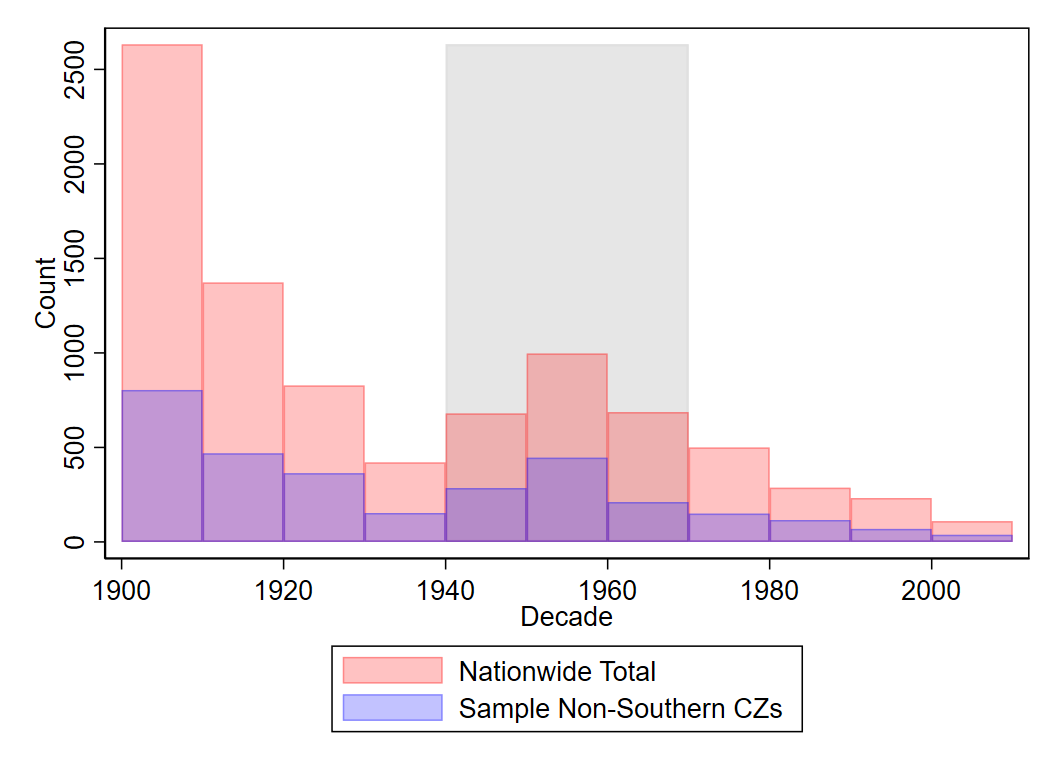
\includegraphics[width = .65\textwidth]{figures/FA1}
   
\end{figure}

\clearpage
\begin{figure*}[htbp]
    \centering
    \caption{Leave-one-out IV Tests, Balanced Controls}
    \begin{subfigure}{0.4\textwidth}
        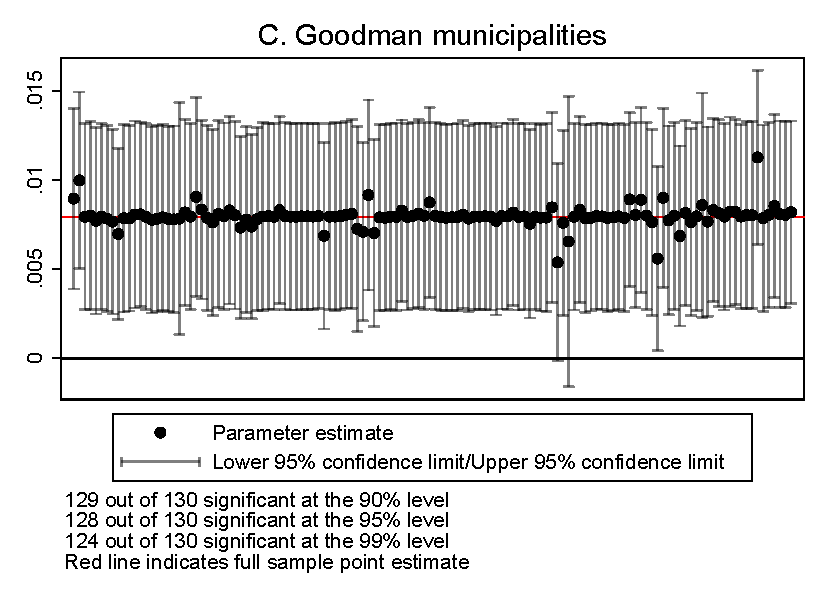
\includegraphics[width=\linewidth]{figures/FA2_cgoodman.pdf}
        \label{fig:sub1}
    \end{subfigure}
    \begin{subfigure}{0.4\textwidth}
        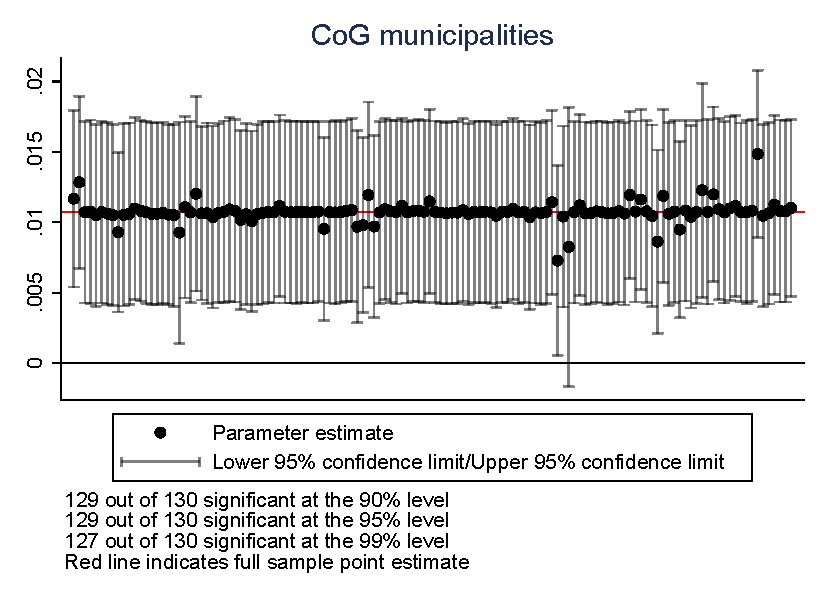
\includegraphics[width=\linewidth]{figures/FA2_gen_muni.pdf}
        \label{fig:sub2}
    \end{subfigure}
    \begin{subfigure}{0.4\textwidth}
        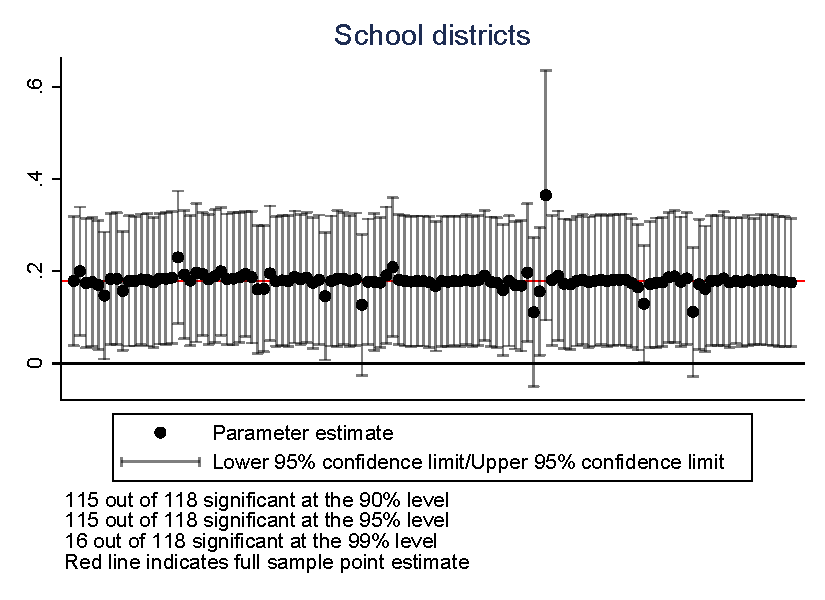
\includegraphics[width=\linewidth]{figures/FA2_schdist_ind.pdf}
        \label{fig:sub3}
    \end{subfigure}
    \begin{subfigure}{0.4\textwidth}
        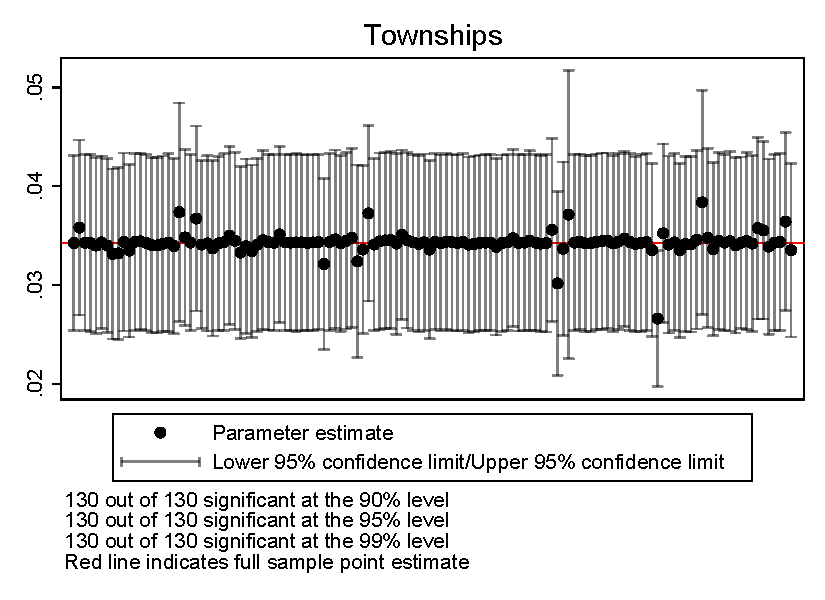
\includegraphics[width=\linewidth]{figures/FA2_gen_town.pdf}
        \label{fig:sub4}
    \end{subfigure}
    \begin{subfigure}{0.4\textwidth}
        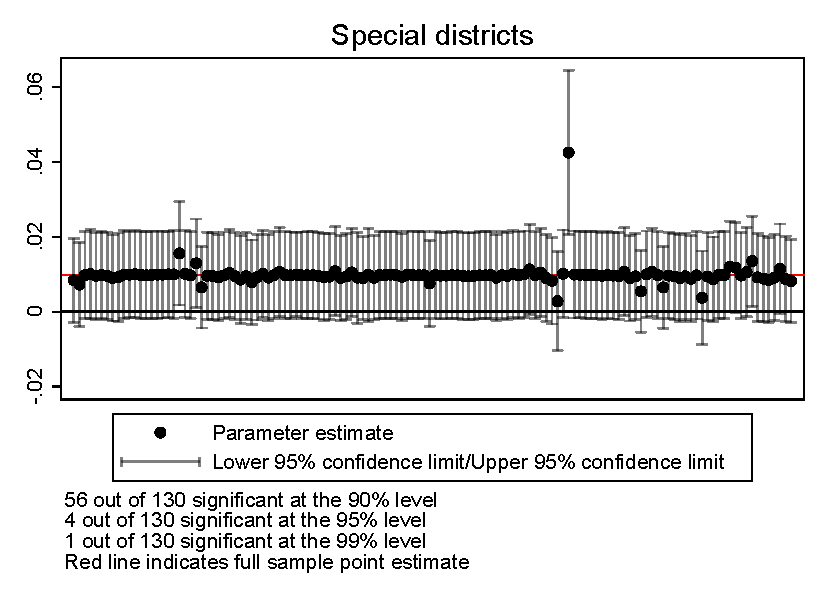
\includegraphics[width=\linewidth]{figures/FA2_spdist.pdf}
        \label{fig:sub5}
    \end{subfigure}
    \begin{subfigure}{0.4\textwidth}
        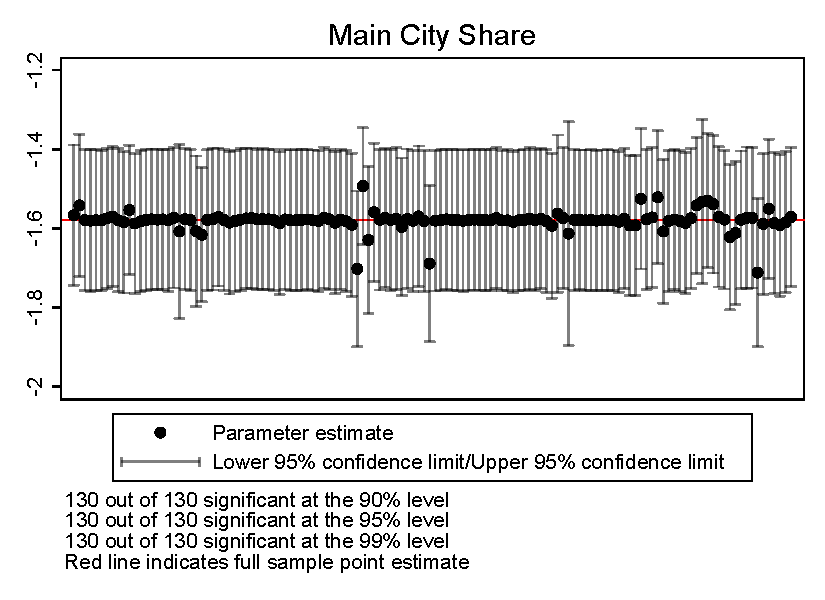
\includegraphics[width=\linewidth]{figures/FA2_totfrac.pdf}
        \label{fig:sub6}
    \end{subfigure}
    \label{fig:loo_iv}
   
\end{figure*}

\clearpage


\begin{figure*}[htbp]
    \centering
    \caption{Overidentification IV Tests, Balanced Controls}
    \begin{subfigure}{0.4\textwidth}
        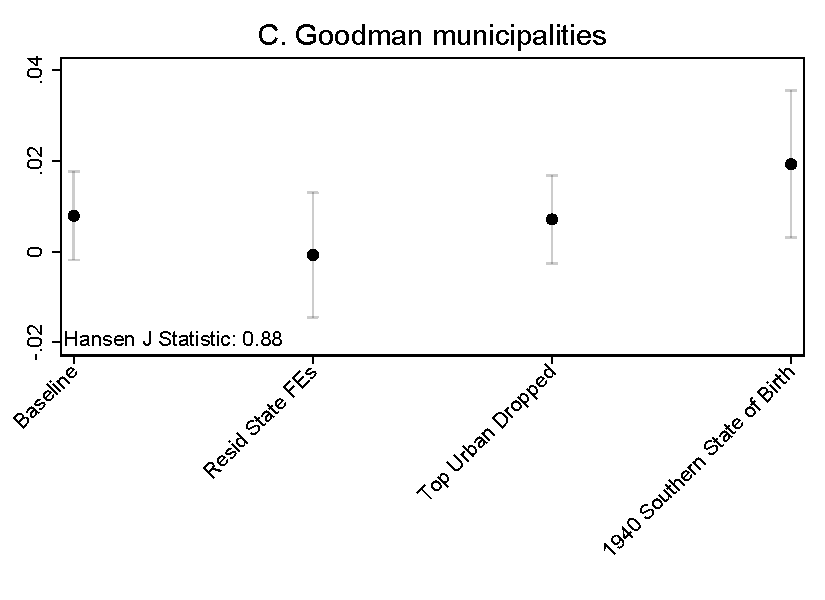
\includegraphics[width=\linewidth]{figures/FA3_cgoodman.pdf}
        \label{fig:sub1}
    \end{subfigure}
    \begin{subfigure}{0.4\textwidth}
        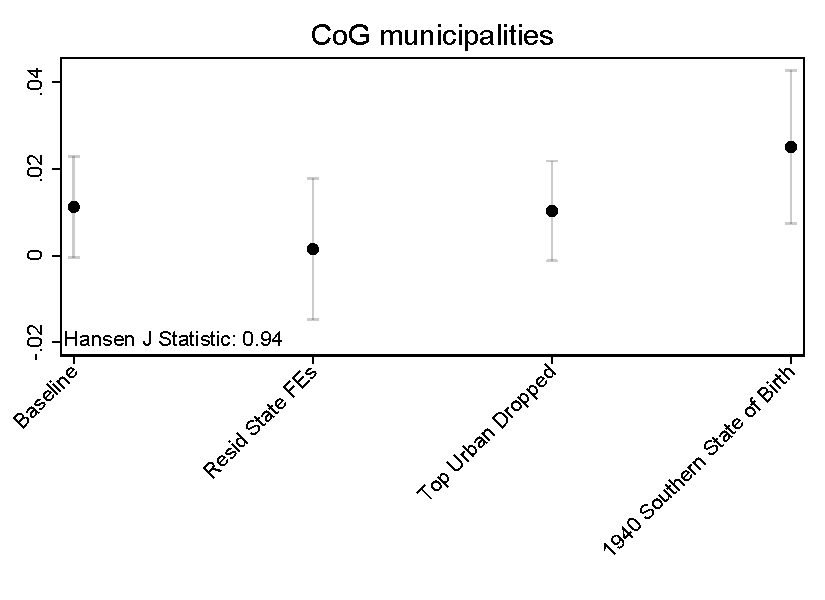
\includegraphics[width=\linewidth]{figures/FA3_gen_muni.pdf}
        \label{fig:sub2}
    \end{subfigure}
    \begin{subfigure}{0.4\textwidth}
        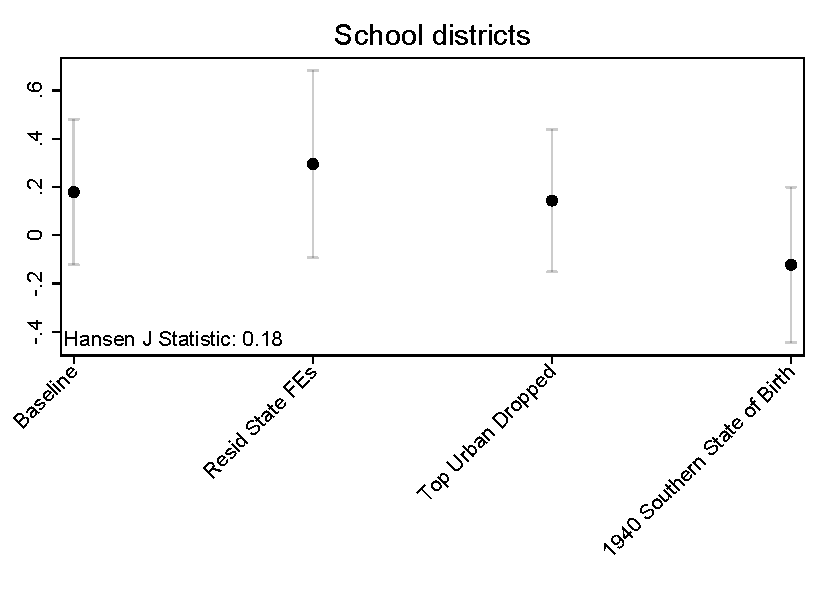
\includegraphics[width=\linewidth]{figures/FA3_schdist_ind.pdf}
        \label{fig:sub3}
    \end{subfigure}
    \begin{subfigure}{0.4\textwidth}
        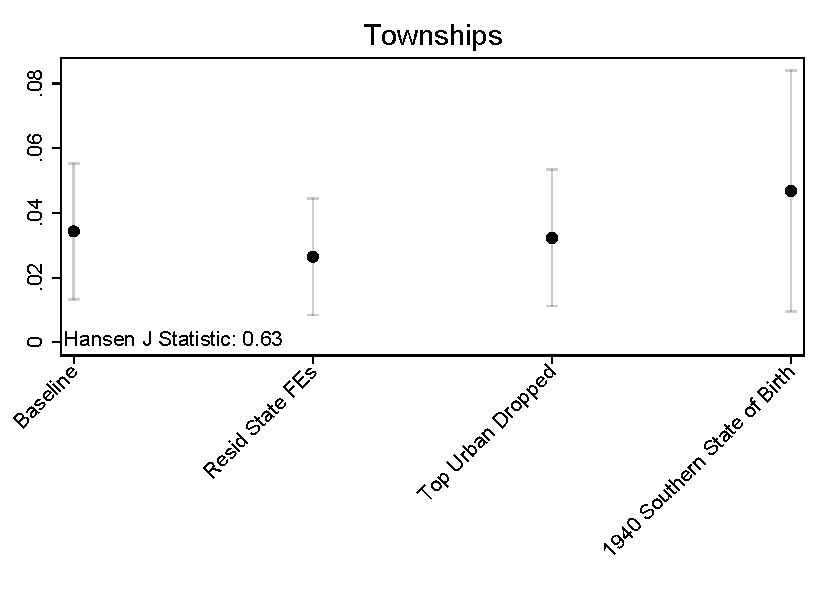
\includegraphics[width=\linewidth]{figures/FA3_gen_town.pdf}
        \label{fig:sub4}
    \end{subfigure}
    \begin{subfigure}{0.4\textwidth}
        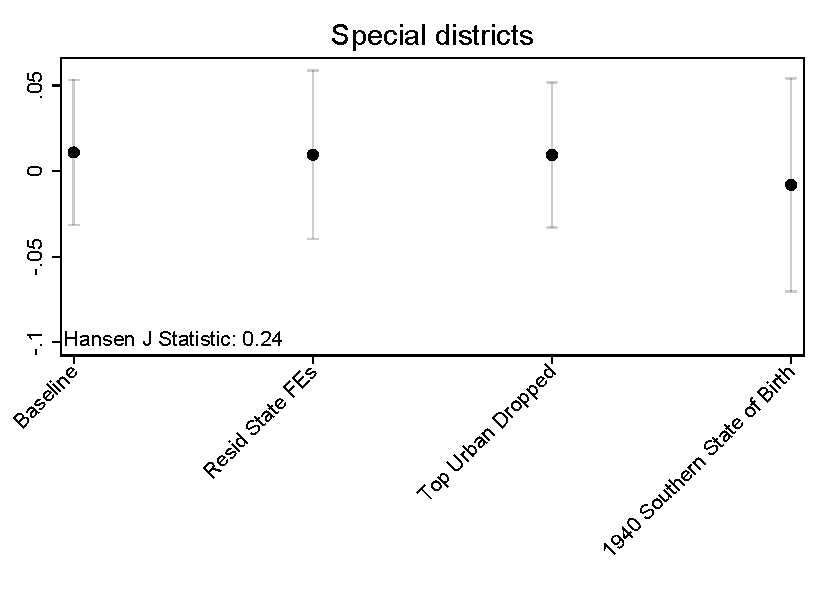
\includegraphics[width=\linewidth]{figures/FA3_spdist.pdf}
        \label{fig:sub5}
    \end{subfigure}
    \begin{subfigure}{0.4\textwidth}
        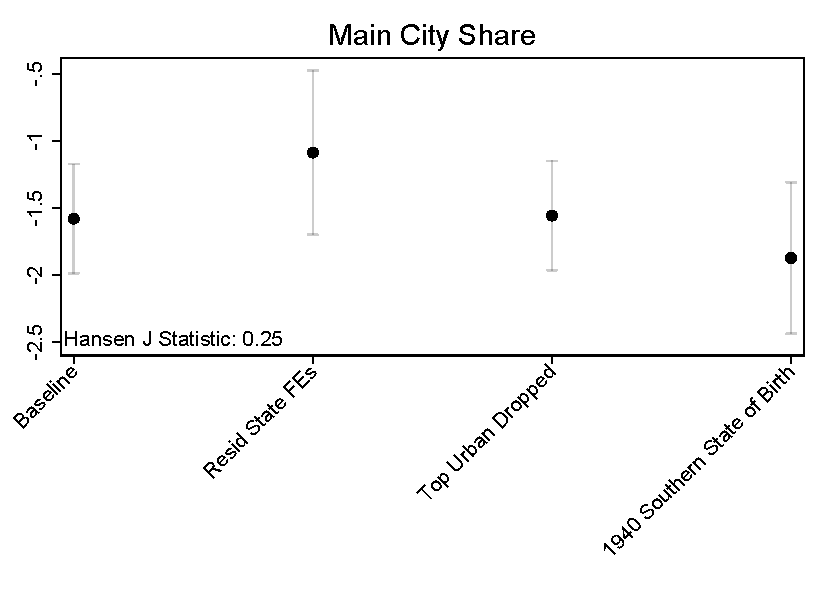
\includegraphics[width=\linewidth]{figures/FA3_totfrac.pdf}
        \label{fig:sub6}
    \end{subfigure}
    \label{fig:alt_inst}
    
\end{figure*}

\clearpage

\begin{figure*}[htbp]
    \centering
    \caption{Placebo Tests, Balanced Controls}
    \begin{subfigure}{0.4\textwidth}
        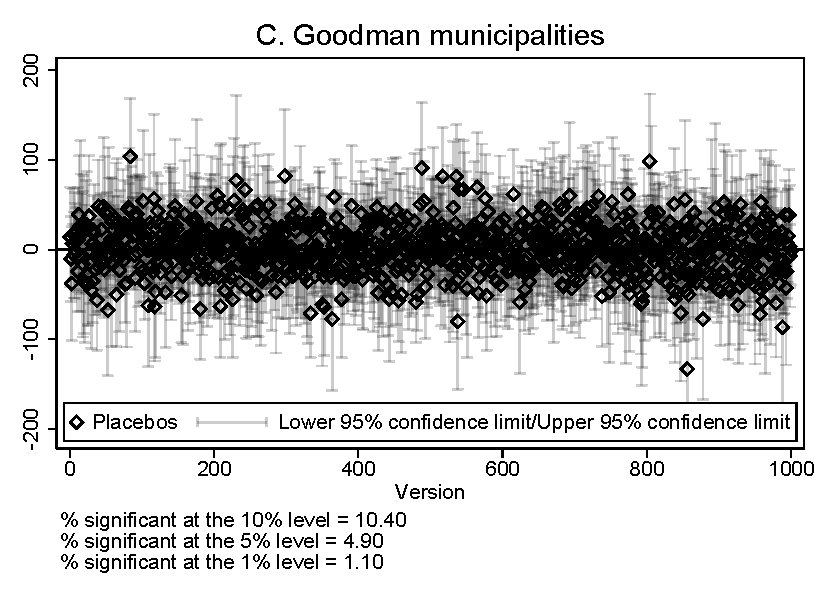
\includegraphics[width=\linewidth]{figures/FA4_cgoodman.pdf}
        \label{fig:sub1}
    \end{subfigure}
    \begin{subfigure}{0.4\textwidth}
        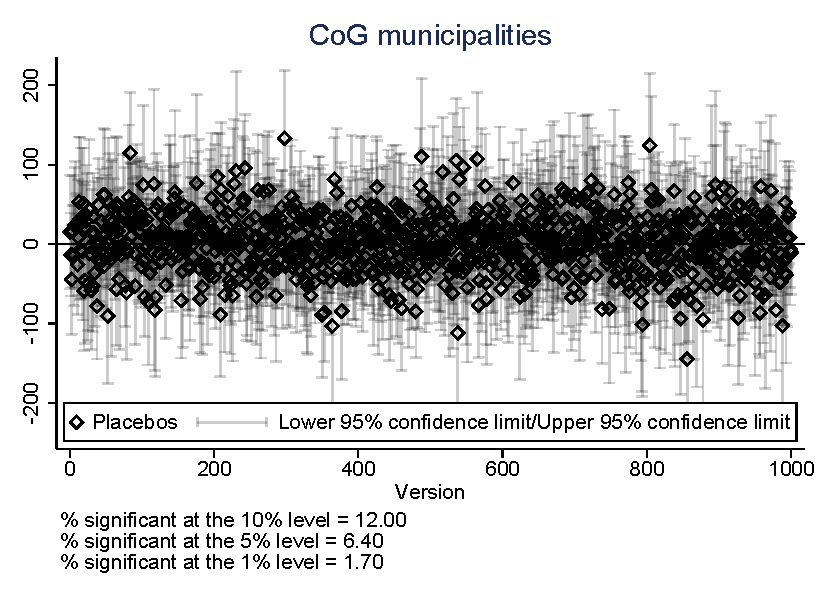
\includegraphics[width=\linewidth]{figures/FA4_gen_muni.pdf}
        \label{fig:sub2}
    \end{subfigure}
    \begin{subfigure}{0.4\textwidth}
        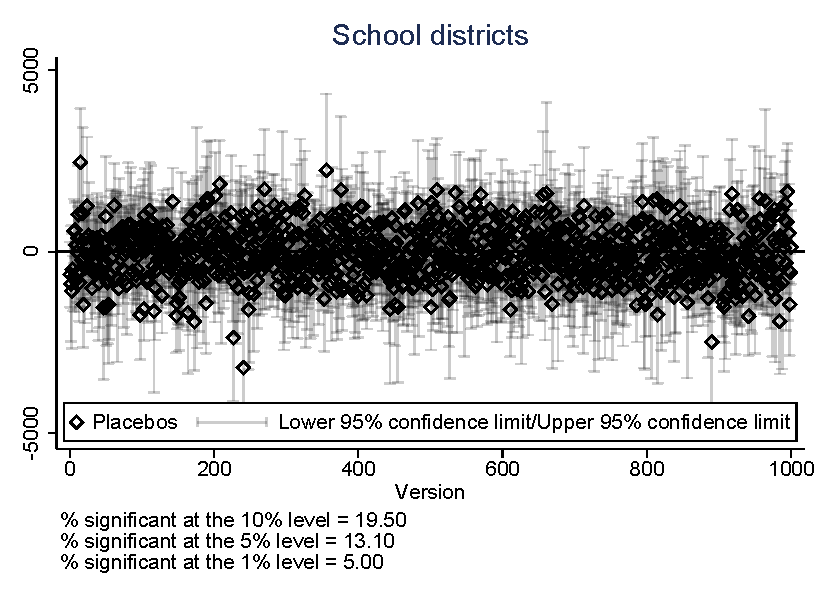
\includegraphics[width=\linewidth]{figures/FA4_schdist_ind.pdf}
        \label{fig:sub3}
    \end{subfigure}
    \begin{subfigure}{0.4\textwidth}
        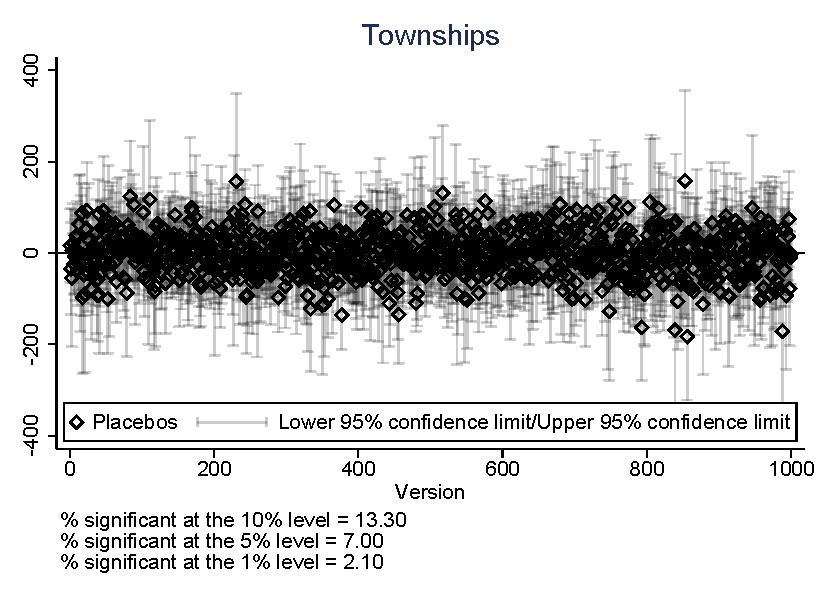
\includegraphics[width=\linewidth]{figures/FA4_gen_town.pdf}
        \label{fig:sub4}
    \end{subfigure}
    \begin{subfigure}{0.4\textwidth}
        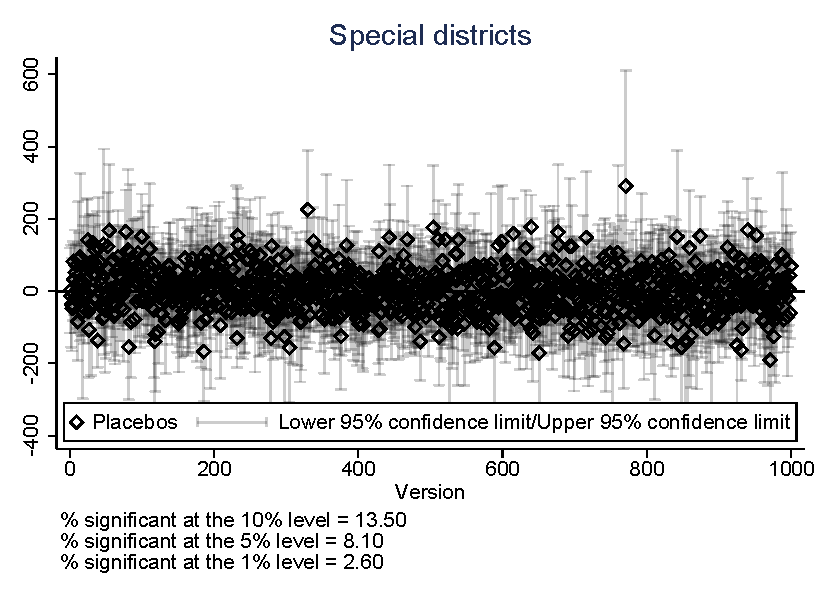
\includegraphics[width=\linewidth]{figures/FA4_spdist.pdf}
        \label{fig:sub5}
    \end{subfigure}
    \begin{subfigure}{0.4\textwidth}
        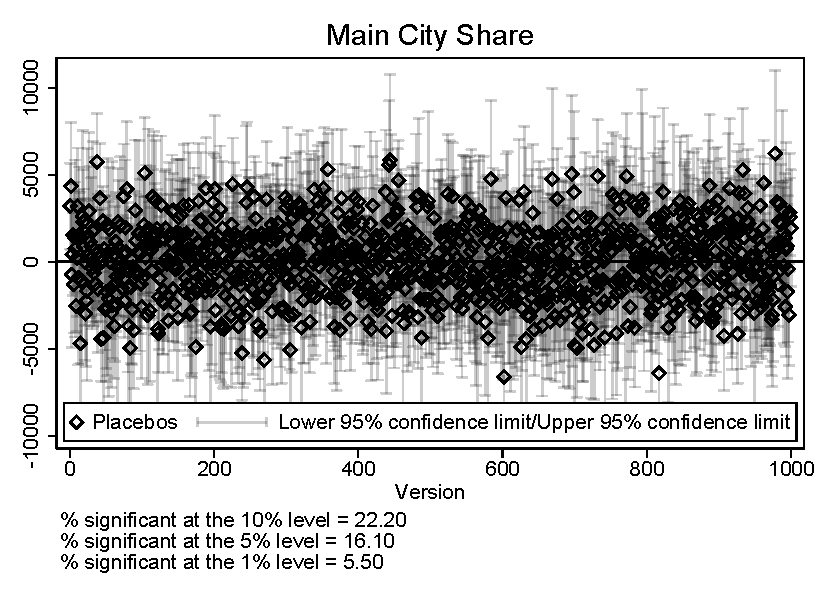
\includegraphics[width=\linewidth]{figures/FA4_totfrac.pdf}
        \label{fig:sub6}
    \end{subfigure}
    \label{fig:placebo}
   
\end{figure*}

\pagebreak
\begin{figure*}[htbp]
    \centering
    \vspace{2cm}
    \caption{Distribution of Distance to Central City, 1940-70 Incorporations}
    \begin{subfigure}{0.6\textwidth}
    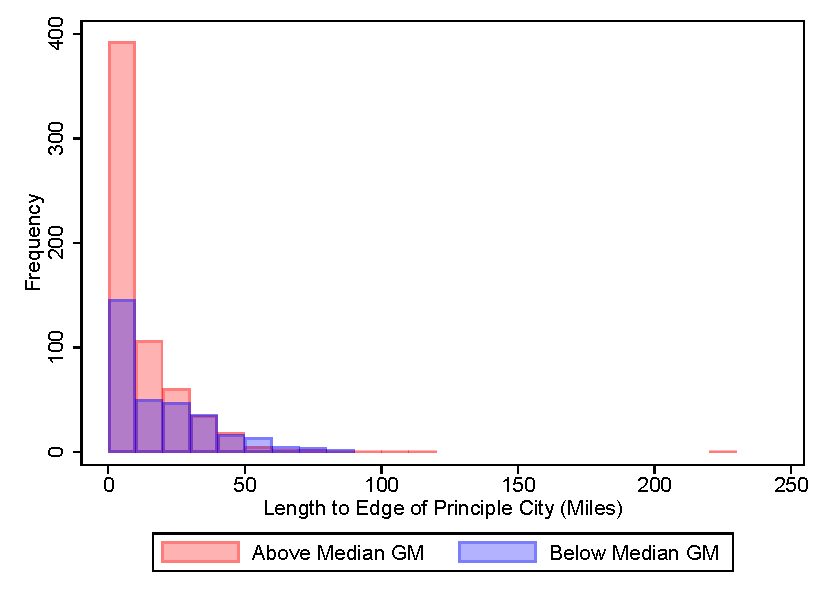
\includegraphics[width=\linewidth]{figures/FA5a}
        \label{fig:sub1}
    \end{subfigure}
    \begin{subfigure}{0.6\textwidth}
        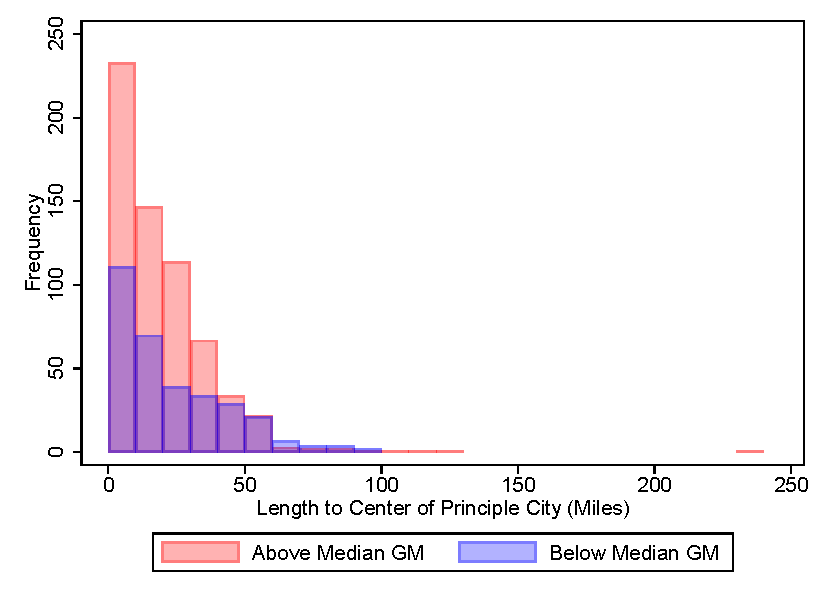
\includegraphics[width=\linewidth]{figures/FA5b.pdf}
        \label{fig:sub2}
    \end{subfigure}
    \label{fig:dist_4070}
    
\end{figure*}

\end{landscape}

\end{document}